% Copyright (C) 2001, International Business Machines
% Corporation, Ted Ralphs and others. All Rights Reserved.

\documentclass[openany,twoside,11pt]{book}

\setlength{\parindent}{0in}
\setlength{\parskip}{0.15in}
\setlength{\oddsidemargin}{0.5in}
\setlength{\evensidemargin}{0in}
\setlength{\topmargin}{0in}
\setlength{\textwidth}{6in}

\usepackage{mathenv}
\usepackage{graphicx}
%\usepackage{epsfig}

\newcommand{\be}{\begin{enumerate}}
\newcommand{\ee}{\end{enumerate}}
\newcommand{\bc}{\begin{center}}
\newcommand{\ec}{\end{center}}
\newcommand{\bt}{\begin{tabular}}
\newcommand{\et}{\end{tabular}}
\newcommand{\bd}{\begin{description}}
\newcommand{\ed}{\end{description}}
\newcommand{\bi}{\begin{itemize}}
\newcommand{\ei}{\end{itemize}}
\newcommand{\bv}{\begin{verbatim}}
\newcommand{\ev}{\end{verbatim}}
\newcommand{\functiondef}[1]{\subsubsection{#1}}

\renewcommand{\functiondef}[1]{\item[\Large $\triangleright$] {\bf \Large #1}}
\newcommand{\describe}{\item[Description:] \hfill}
\newcommand{\args}{\item[Arguments:] \hfill}
\newcommand{\returns}{\item[Return values:] \hfill}
\newcommand{\postp}{\item[Post-processing:] \hfill}
\newcommand{\nopostp}{\item[Post-processing:] None \hfill}

\newcommand{\BB}{{\sc COIN/BCP}}
\newcommand{\TM}{{\sc TreeManager}}
\newcommand{\LP}{{\sc LP}}
\newcommand{\ra}{$\rightarrow$}

\newcommand{\eqsep}{\hspace{.25em}}
\newcommand{\commentout}[1]{}
\newcommand{\code}[1]{{\tt #1}}

\begin{document}

\title{\BB\ User's Manual}
\author{
T.K. Ralphs\thanks{Department of Industrial and Manufacturing Systems 
Engineering, Lehigh University, Bethlehem, PA 18015, {\tt
tkralphs@lehigh.edu}, {\tt http://www.lehigh.edu/\~{ }tkr2}} 
\and
L. Lad\'anyi\thanks{Department of Mathematical Sciences, 
IBM T.J. Watson Research Center, Yorktown Heights,
NY 10598} \\
}
\date{January 2001}
\maketitle

\newpage

\thispagestyle{empty}

\vspace*{3in}
\begin{center}
{\copyright 2001 International Business Machines Corporation, Ted
Ralphs and others. All right reserved.}
\end{center}

\newpage

\tableofcontents

%%%%%%%%%%%%%%%%%%%%%%%%%%%%%%%%%%%%%%%%%%%%%%%%%%%%%%%%%%%%%%%%%%%%%%%%%%%%%%
% Insert here the references that are not referred to anywhere, but we want
% them to be listed anyway.
%%%%%%%%%%%%%%%%%%%%%%%%%%%%%%%%%%%%%%%%%%%%%%%%%%%%%%%%%%%%%%%%%%%%%%%%%%%%%%

\begin{tabbing}
%\cite{B:ahuja-magnanti-orlin} \kill
%\cite{B:cook-lovasz-seymour} \kill
\end{tabbing}

%%%%%%%%%%%%%%%%%%%%%%%%%%%%%%%%%%%%%%%%%%%%%%%%%%%%%%%%%%%%%%%%%%%%%%%%%%%%%%

\chapter{Introduction}
\label{man-intro}
\section{A Brief History}

Since the inception of optimization as a mathematical discipline,
researchers have been intrigued and stymied by the
difficulty of solving discrete
optimization problems. Even problems with natural and concise formulations
remain 
challenging to solve in practice. The most significant advance in general
methodologies occured in 1991 when Padberg and Rinaldi
\cite{A:padberg-rinaldi} merged the enumeration approach of branch and bound
algorithms with the polyhedral approach of cutting planes to create
the technique we call {\em branch, cut
and price} or simply {\em BCP}. 
Integrating the contributions of many in the field , their paper launched a
new era in discrete optimization techniques.

In the last two decades, we have seen tremendous progress in our
ability to solve specially structured large-scale discrete 
optimization problems. Indeed,
in 1998, Applegate, Bixby, Cook, and Chv\'atal \cite{W:concorde}
solved a {\em Traveling
Salesman Problem} (TSP) instance with 13,509 cities; a full order of
magnitude larger than what had been possible just a decade earlier
and two orders of magnitude larger than the largest
problem that had been solved up until 1978. This progress becomes even
more impressive when one realizes that the number of variables in the
standard formulation for this problem is approximately the {\em
square} of the problem size. Hence, we are talking about solving a
problem with somewhere in excess of {\em 100 million variables}.

This fantastic progress can be attributed to several factors. 
The increase in available computing power over the last decade, both
in terms of processor speed and memory, has been nothing short of
amazing. This hardware improvement made it possible to tackle larger problems
thus accumulating knowledge about how the large problems ``behave''. In turn,
this led to increasingly sophisticated software for
optimization, and to a wealth of theoretical results.
Also, many theoretical results, which had no computational importance for
small problems, were ``re-discovered'' as larger problems
became the target. Finally, the use of
parallel computing has allowed researchers to further leverage their
gains.

As computational research in optimization becomes more widespread and
the sophistication of computational techniques increases, 
one of the main difficulties faced by researchers in the area
is the level of effort required to
develop an efficient implementation. The need for
incorporating problem-dependent methods (most notably dynamic
generation of variables and cutting planes) typically required
time-consuming development of custom implementations. In the early 1990's
a research group was formed with the goal of creating 
a generic software framework which users
could easily customize for their particular problem class. This
group eventually produced what was then known as COMPSys
(Combinatorial Optimization Multi-processing System) \cite{P:compsys}. 
After several
revisions which broadened the framework's functionality, 
COMPSys became SYMPHONY
(Single- or Multi-Process Optimization over Networks)
\cite{W:symphony}. Starting in 1998 a total reimplementation in C++ was
undertaken at IBM research to enable greater flexibility. The result of this
effort was opened up as an open-source project in 2000 under the auspices of
the Common Optimization INterface for Operations Research (COIN-OR) 
\cite{W:coin-or} and is codenamed \BB.

\section{Related Work}

In the 1990's, there was a virtual explosion of software for discrete
optimization. Almost without exception, these new software packages
were based on the basic techniques of branch, cut and price. The
general-purpose packages fall into two main
categories -- those based on algorithms not exploing special structures 
for solving general
mixed integer programs (MIPs)
and those facilitating the use of special structure via
user-supplied, problem-specific subroutines. We will call
packages in this second category {\em frameworks}. There have also been
numerous special-purpose codes developed specifically for use in a
particular problem setting. 

Of the two categories, general-purpose MIP solvers are the most common. 
Among the 
dozens of offerings in this category, the most notable are MINTO
\cite{W:minto}, MIPO \cite{W:mipo}, bc-opt \cite{W:bcopt} and 
several commercial
packages. 

Generic
frameworks, on the other hand, are far less numerous. The most full-featured
packages available are the two frameworks we have already mentioned (SYMPHONY
and \BB) and a commercial product, ABACUS \cite{W:abacus}.
Some general-purpose MIP solver, such as
MINTO \cite{W:minto} and several commercial packages, now have a limited
capability of utilizing problem-specific subroutines.

Related software includes general MIP solvers implementing
parallel branch and bound (PARINO \cite{W:parino} and FATCOP
\cite{W:fatcop}); frameworks for general parallel branch and 
bound (PUBB \cite{W:pubb}, BoB \cite{W:bob}, PPBB-Lib
\cite{W:ppbb-lib}, and PICO \cite{W:pico}) and special-purpose codes, like 
CONCORDE, a package for solving the {\em Traveling Salesman Problem}
(TSP). This latter code is the  most sophisticated special-purpose
code developed to date.

%If the objective function $f$ is linear, and the set $S$
%consists of $n$-dimensional vectors, then it is sufficient to 

%and are
%important both from a practical and a theoretical perspective. 
%and Integer Programming have always been
%important application areas
%Although parallel computation has been a hot research topic for a
%number of years, few researchers have been devoted to solving 
%hard discrete ongoing in the computer
%science community for years, very little of the knowledge that has
%been developed in that community has made the crossover to
%applications in other fields. This is especially true for Operations
%Research in general and discrete optimization specifically, where many
%problems lend themselves naturally to to parallelization.

%Throughout the 1990's, the pace of change in computing was more rapid
%than ever before. Faster chips, more memory, and better software were
%were a demanded by businesses who wanted to keep their competitive
%edge. Customers insisted on faster, better service and Web servers had to
%deal with an ever increasing desire for information. In the face of
%this increasing need for computing power, many companies began to turn to
%multi-processor servers as an economical alternative to buying and
%networking multiple single-processor computers. Today, small
%shared-memory parallel computers are common-place in many companies.
%Most large vendors now offer multi-processor servers as a mainstay of
%their high-end product lines. We are now entering the age of parallel
%computing.

%During the coming decade, the pace of development of both hardware and
%software that can take advantage of parallelism to deliver superior
%computing performance will no doubt increase. Research in application
%areas such as discrete optimization will help spur this development
%and allow the US to maintain it's competitive edge in world markets. 

\section{Organization of the Manual}

The manual is divided into three parts. Part I is a gentle
introduction to branch, cut and price algorithms, including an
overview of the design of \BB. Anyone interested in learning
about or using the framework should spend time with Part I;
those already familiar with BCP algorithms will probably want to skim
the introductory sections. The reader merely
interested in only a high-level description of the framework may wish to
stop after reading Part I. Part II
is intended to provide the specific details needed
to actually develop applications using \BB. This includes ``how-to''
descriptions of customizing the Makefiles, compiling the sample code, deciding
wich built-in methods to override, 
and performing other development tasks such as
debugging. Part III illustrates these principles with a concrete
example. A reference manual of every class structure is available in
HTML format and is part of the standard distribution.

\section{Introduction to Branch, Cut and Price}
\label{B&C-intro}

\subsection{Branch and Bound}

{\em Branch and bound} is the broad class of algorithms from which
branch, cut and price is descended. A branch and bound algorithm uses
a divide and conquer strategy; it partitions the solution space into
{\em subproblems} and then optimizes over each subproblem 
individually. For instance, let $S$ be the set of solutions to a given
problem, and let $c \in {\bf R}^S$ be a vector of costs associated
with members of S. Suppose we wish to determine a least cost member of
S and we are given $\hat{s} \in S$, a ``good'' solution determined
heuristically. Whenever a new, better solution is found we will replace 
$\hat{s}$ with the new solution. Thus the value of $\hat{s}$ is always a
{\em global upper bound} on th eoptimal value.
In the branch and bound algorithm we maintain a list of 
{\em candidate subproblems} each of which contain 
a subset of the original feasible solutions. This list is
initialized by placing $S$ on it.
In the {\em processing} or {\em bounding} phase of the algorithm we take 
an entry, say $S'$. from the candidate list and remove it from the list.
We {\em relax} $S'$, that is, we admit solutions that are not in $S'$ and
solve the relaxd problem. There are four possible results. 
\begin{itemize}
\item The relaxed problem is found to be infeasible. In this case we 
  obviously cannot find a new feasible solution that is feasible and is in 
  $S'$, thus we can {\em prune} (or {\em fathom}) the subproblem, that is, we
  discard it.
\item The optimal solution to the relaxed problem is not better 
  (not lower) than the global upper bound. In this case the value of any
  feasible solution in $S'$ must also not be better than the global upper
  bound thus we cannot find a feasible solution in $s'$ that would be better
  than the currently known best solution. Therefore we can fathom the 
  subproblem in this case, too.
\item The optimal solution to the relaxed problem is better than the global
  upper bound {\em and} it is in $S'$, i.e., it is feasible. In this case we
  replace $\hat{s}$ with this new solution. Also, we cannot find any even
  better solution in this subproblem thus we can fathom it.
\item The optimal solution to the relaxed problem is better than the global
  upper bound but is not in $S'$. In this case we {\em branch}, i.e., we 
  identify $n$ subsets of 
  $S'$, $S'_1, \ldots, S'_n$, such that $\cup_{i = 1}^n S'_i = S'$. 
  Each of these subsets, the {\em children} of $S'$, is a new candidate
  subproblem and is added to the candidate list. 
\end{itemize}
After a subproblem is processed (and either pruned or branched) a new
subproblem is 
selected for processing as long as the candidate list is not empty, at 
which point our current best solution is the optimal one.

%Using branch and bound, we initially examine the entire
%solution space $S$. In the {\em processing} or {\em bounding} phase,
%we relax the problem. In so doing, we admit solutions that are not in
%the feasible set $S$. Solving this relaxation yields a lower bound on
%the value of an optimal solution. If the solution to this relaxation
%is a member of $S$ or has cost equal to $\hat{s}$, then we are
%done -- either the new solution or $\hat{s}$, respectively, is optimal.
%Otherwise, we identify $n$ subsets of $S$, $S_1, \ldots, S_n$, such
%that $\cup_{i = 1}^n S_i = S$. Each of these subsets is called a {\em
%subproblem}; $S_1, \ldots, S_n$ are sometimes called the {\em
%children} of $S$. We add the children of $S$ to the list of {\em
%candidate subproblems} (those which need processing). This is called
%{\em branching}.

%To continue the algorithm, we select one of the candidate subproblems
%and process it. There are four possible results. If we find a feasible
%solution better than $\hat{s}$, then we replace $\hat{s}$ with the new
%solution and continue. If we find that the subproblem has no
%solutions we discard, or {\em prune} (or {\em fathom} it.
%Otherwise, we
%compare the lower bound to our global upper bound. If it is greater
%than or equal to our current upper bound, then we can prune the
%subproblem. Finally, if we cannot prune the subproblem, we are forced
%to branch and add the children of this subproblem to the list of
%active candidates. We continue in this way until the list of active
%subproblems is empty, at which point our current best solution is the
%optimal one.

The sequence of subproblems generated can be displayed as a rooted directed
graph; the original problem being the root and there are edges from each
subproblem to its children. This graph is the {\em search tree} and the
expression {\em search (tree) node} is used interchangeably with 
{\em subproblem}.

In many applications, the bounding operation is accomplished using the
tools of linear programming (LP), a technique first described in full
generality by Hoffman and Padberg \cite{A:hoffman-padberg}. This general 
class of 
algorithms is known as {\em LP-based branch and bound}. Typically, the
integrality constraints of an integer programming formulation of the
problem are relaxed to obtain a {\em LP relaxation}, which is then
solved to obtain a lower bound for the problem.

\subsection{Branch and Cut}
\label{branchandcut}

Padberg and Rinaldi \cite{A:padberg-rinaldi} improved on the basic idea of 
LP-based branch and 
bound by describing a method
of using globally valid inequalities (i.e., inequalities valid for the
convex hull of integer solutions) to strengthen the LP relaxation.
They called this technique {\em branch and cut}. Since then, many
implementations (including ours) have been fashioned around the
framework they described for solving the Traveling Salesman Problem.

As an example, let a combinatorial optimization problem $\hbox{\em CP} =
(E, {\cal F})$ with {\em ground set} $E$ and {\em feasible set} ${\cal F}
\subseteq 2^E$ be given along with a cost function $c \in {\bf R}^E$.
Now let ${\cal P}$ be the convex hull of incidence vectors of members of 
${\cal F}$. Then we know by Weyl's Theorem (see \cite{B:nemhauser-wolsey}) 
that there 
exists a finite set of inequalities ${\cal L}$ which are valid for 
${\cal P}$ such that
\begin{equation}
\label{the-polyhedron}
{\cal P} = \{x \in {\bf R}^n: ax \leq \beta\;\;\forall\;(a, \beta) \in 
{\cal L}\}.
\end{equation}
Unfortunately, it is usually
difficult, if not impossible, to enumerate all inequalities in
${\cal L}$ (or even just those that describe the convex hull near the 
optimal corner) or we could simply solve the problem using linear
programming.

The set of incidence vectors corresponding to the members of ${\cal F}$ is
sometimes approximated as the set of all incidence vectors obeying a
(relatively) small set of inequalities (these inequalities are
typically the ones used in the initial LP relaxation). Then in each node of
the search tree globally valid inequalities are generated (the best such
inequalities are in ${\cal L}$) using separation algorithms and heuristics.
One could say that the inequalities describing ${\cal P}$ are defined
implicitely and generated as they are needed.

This way the relaxation is tightened thus the bounding step has a better
chance to fathom the node based on the objective value.
In Figure \ref{proc-bound}, we describe more
precisely how cut generation is employed within the bounding operation 
of the branch and cut technique.

\begin{figure}
\framebox[5.75in]{
\begin{minipage}{5.25in}
\vskip .1in
{\rm
{\bf Bounding Operation}\\
\underbar{Input:} A subproblem ${\cal S}$, described in
terms of a ``small'' set of inequalities ${\cal L'}$ such that ${\cal
S} = \{x^s : s \in {\cal F}\;\hbox{\rm and}\;ax^s \leq \beta\;\forall
\;(a,\beta) \in {\cal L'}\}$ and $\alpha$, an upper bound on the global 
optimal value. \\
\underbar{Output:} Either (1) an optimal solution $s^* \in {\cal S}$ to
the subproblem, (2) a lower bound on the optimal value of the 
subproblem, or (3) a message {\tt pruned} indicating that the
subproblem should not be considered further. \\
{\bf Step 1.} Set ${\cal C} \leftarrow {\cal L'}$. \\ 
{\bf Step 2.} Solve the LP $\min\{cx : ax \leq \beta\;\forall\;(a, \beta) 
\in {\cal C}\}$. \\
{\bf Step 3.} If the LP has a feasible solution $\hat{x}$, then go to
Step 4. Otherwise, STOP and output {\tt pruned}. This subproblem has no 
feasible solutions. \\ 
{\bf Step 4.} If $c\hat{x} < \alpha$, then go to Step
5. Otherwise, STOP and output {\tt pruned}. This subproblem
cannot produce a solution of value better than $\alpha$. \\ 
{\bf Step 5.} If $\hat{x}$ is the incidence vector of some $\hat{s}
\in {\cal S}$, then $\hat{s}$ is the optimal solution to this
subproblem. STOP and output $\hat{s}$ as $s^*$. Otherwise, apply
separation algorithms and heuristics to $\hat{x}$ to get a set of
violated inequalities ${\cal C'}$. If ${\cal C'} = \emptyset$, then
$c\hat{x}$ is a lower bound on the value of an optimal element of
${\cal S}$.  STOP and return $\hat{x}$ and the lower bound
$c\hat{x}$. Otherwise, set ${\cal C} \leftarrow {\cal C} \cup {\cal
C'}$ and go to Step 2.}
\end{minipage}
}
\caption{Bounding in the branch and cut algorithm}
\label{proc-bound}
\end{figure}

Once we have failed to generate cuts and the subproblem still cannot be pruned
based on the objective value, we are forced to
branch. The branching operation is accomplished by specifying a set of
hyperplanes which divide the current subproblem in such a way that the
current solution is not feasible for the LP relaxation of any of the
new subproblems. For example, in a combinatorial optimization problem,
branching could be accomplished simply by fixing a variable whose
current value is fractional to 0 in one branch and 1
in the other. The procedure is described more formally in Figure
\ref{branching-fig}. Figure \ref{gb&c} gives a high level description
of the generic branch and cut algorithm.

\begin{figure}
\framebox[5.75in]{
\begin{minipage}{5.25in}
\vskip .1in
{\rm
{\bf Branching Operation} \\
\underbar{Input:} A subproblem ${\cal S}$ and $\hat{x}$, the LP solution
yielding the lower bound. \\
\underbar{Output:} $S_1, \ldots, S_p$ such that ${\cal S} = \cup_{i = 1}^p
S_i$. \\
{\bf Step 1.} Determine sets ${\cal L}_1, \ldots, {\cal L}_p$ of
inequalities such that ${\cal S} = \cup_{i = 1}^n \{x \in {\cal S}: ax \leq
\beta\;\forall\;(a, \beta) \in {\cal L}_i\}$ and $\hat{x} \notin
\cup_{i = 1}^n S_i$. \\
{\bf Step 2.} Set $S_i = \{x \in {\cal S}: ax \leq
\beta\;\;\forall\;(a, \beta) \in {\cal L}_i \cup {\cal L}'\}$ where 
${\cal L'}$ is the set of inequalities used to describe ${\cal S}$.}
\end{minipage}
}
\caption{Branching in the branch and cut algorithm}
\label{branching-fig}
\end{figure}

\begin{figure}
\framebox[5.75in]{
\begin{minipage}{5.25in}
\vskip .1in
{\rm
{\bf Generic Branch and Cut Algorithm}\\
\underbar{Input:} A data array specifying the problem instance.\\
\underbar{Output:} The global optimal solution $s^*$ to the problem
instance. \\
{\bf Step 1.} Generate a ``good'' feasible solution ${\hat s}$ using 
heuristics. Set $\alpha \leftarrow c(\hat{s})$. \\
{\bf Step 2.} Generate the first subproblem ${\cal S}^I$ by constructing a
small set ${\cal L'}$ of inequalities valid for ${\cal P}$. Set $A
\leftarrow \{{\cal S}^I\}$. \\
{\bf Step 3.} If $A = \emptyset$, STOP and output $\hat{s}$ as the
global optimum $s^*$. Otherwise, choose some ${\cal S} \in A$. Set $A
\leftarrow A \setminus \{{\cal S}\}$. Process ${\cal S}$. \\
{\bf Step 4.} If the result of Step 3 is a feasible solution
$\overline{s}$, then $c\overline{s} < c\hat{s}$.
Set $\hat{s} \leftarrow \overline{s}$ and $\alpha \leftarrow 
c(\overline{s})$ and go to Step 3. If the subproblem was pruned, go to
Step 3. Otherwise, go to Step 5. \\
{\bf Step 5.} Perform the branching operation. Add the set of
subproblems generated to $A$ and go to Step 3.}
\end{minipage}
}
\caption{Description of the generic branch and cut algorithm}
\label{gb&c}
\end{figure}

Note that adding cutting planes only increases the lower bound at a search
tree node hence as soon as the lower bound on a node exceeds the value of the
best known solution the search tree node can be fathomed.

\subsection{Branch and Price}
\label{branchandprice}

As with cutting planes, the columns of $A$ can also be defined
implicitly if $n$ is large. If column $i$ is not present in the
current matrix, then variable $x_i$ is implicitly taken to have value
zero. The process of dynamically generating variables is called {\em
pricing} in the jargon of linear programming. The term originates from
computing the {\em reduced cost} of the column and adding the column to the
formulation if it has a negative reduced cost. This procedure
can also be viewed
as that of generating cutting planes for the dual of the current
LP relaxation. Hence, LP-based branch and bound algorithms in which
the variables are generated dynamically when needed are known as {\em
branch and price} algorithms. Savelsbergh,
et al. \cite{branchandprice} provide a thorough review of these methods. 

Although ``branch and cut'' and ``branch and price'' look very symmetric there
is a very significant difference. When cuts are introduced the lower bound on
the relaxation can only increase while introducing new columns can lower the
lower bound. Therefore a search tree node cannot be fathomed until all
variables are priced out {\em and} the lower bound is higher than the best
known solution value. For this reason frequently the {\em price and branch}
algorithm is executed, that is first we price, then we do plain branch and
bound. Obviously, this will most likely result in a suboptimal solution, but
for practical purposes this is usually sufficient.

\subsection{Branch, Cut and Price}
\label{branchandcutandprice}

Finally, when both variables and cutting planes are generated dynamically
during LP-based branch and bound, the technique becomes known as {\em
branch, cut and price} (BCP). In such a scheme, there is a pleasing
symmetry between the treatment of cuts and variables.
However, it is important to note that while branch, cut and
price does combine ideas from both branch and cut and branch and price
(which are very similar to each other anyway), combining the two
techniques requires much more sophisticated methods than either one
requires on its own. The effects of this observation are noticable throughout
the design of \BB\ (see, in particular, Section \ref{data-structures}).

\section{Design of \BB}
\label{design}

\BB\ was designed with three major goals in mind -- portability, 
efficiency and
ease of use. With respect to ease of use, we aimed for a ``black box''
design, whereby the user would not be required to know anything about
the implementation of the library, but only about the user interface.
With respect to portability, we aimed not only for it to be {\em
possible} to use the framework in a wide variety of settings and on a
wide variety of hardware, but also for it to perform {\em effectively} in all
these settings. Our primary measure of effectiveness is
how well the framework performs in comparison to problem-specific
(or hardware-specific) implementation written ``from scratch.''

It is important to point out that achieving such design goals involves
a number of very difficult tradeoffs, which we will highlight
throughout the rest of the manual. For instance, ease of use is quite
often at odds with efficiency. In several instances, we had to give up
some efficiency to make the code easy to work with and to maintain a
true black box implementation. Maintaining portability across a wide
variety of hardware, both sequential and parallel, also required some
difficult choices. For example, solving large-scale problems on
sequential platforms requires extremely memory-efficient data
structures in order to maintain the very large search trees that can
be generated. However, these storage schemes are highly centralized
and do not scale well to large numbers of processors. 

\subsection{An Object-oriented Approach}
\label{object-oriented}

Applying BCP to large-scale problems
presents several difficult challenges. First and foremost is designing
methods and data structures capable of handling the potentially huge
number of global cuts and variables that need to be accounted for
during the solution process. A second challenge, which is closely
related to the first, is effectively dealing with the very large
search trees that can be generated for difficult problem instances. A
third challenge is to deal with these issues using a
problem-independent approach. 
%From this point of view, it quickly
%became evident that the vast majority of the procedures in branch and
%cut that depend on the problem setting have to do with generating,
%manipulating, and storing the cuts and variables.

Describing a node in the search tree consists of, among other things,
specifying which cuts and variables are initially {\em active} in the
subproblem. Hence, the central ``objects'' in our framework
are the cuts and variables. From the user's perspective, implementing
a BCP algorithm using \BB\ consists primarily of specifying
various properties of objects, such as how they are generated, how
they are represented, and how they should be realized within the
context of a particular subproblem. This is achieved using class derivation
and virtual methods. There are a few base classes defined in \BB\ that the
user can derive classes from and then she can override the virtual methods
hence modifying the behavior of the code. Some methods she must override, and
for some she can just let the method in the base class executed thus selecting
the default behavior. 
In Sections \ref{dev:overview-hierarchy} and \ref{dev:user-derived} a more
detailed 
description is given about the classes the user can derive new object types
from. 

\subsection{Data Structures and Storage}
\label{data-structures}

Both the memory required to store the search tree and the time
required to process a node are largely dependent on the number of
objects (cuts and variables) that are active in each subproblem.
Keeping this active set as small as possible is one of the keys to
efficiently implementing BCP. For this reason, we chose data
structures that enhance our ability to efficiently move objects in and
out of the active set. Allowing sets of cuts and variables to move in
and out of the linear programs simultaneously is one of the most
significant challenges of BCP. We do this by maintaining an abstract
{\em representation} of each global object that contains information
about how to add it to a particular LP relaxation. 

In the literature on linear and integer programming, the terms {\em
cut} and {\em row} are typically used interchangeably. Similarly, {\em
variable} and {\em column} are often used with similar meanings. In
many situations, this is appropriate and does not cause confusion.
However, in object-oriented BCP frameworks, such as \BB\ or ABACUS,
a {\em cut} and a {\em row} are {\bf fundamentally different objects}. 
A {\em cut} (also referred to as a {\em
constraint}) is a user-defined representation of an abstract object
which can only be realized as a row in an LP matrix {\bf with respect
to a particular set of active variables}. Similarly, a {\em variable}
is a representation which can only be realized as a column of an LP
matrix {\bf with respect to a particular set of cuts}. This
distinction between the {\em representation} and the {\em realization}
of objects is a crucial design element and is what allows us to
effectively address some of the challenges inherent in BCP. In the
remainder of this section, we will further discuss this distinction
and the details of how it is implemented.

%In later sections, we will discuss the computational issues involved
%in the efficient processing of individual subproblem.

\subsubsection{Variables and Cuts}
\label{variables-cuts}

Although their algorithmic roles are different, variables and cuts as objects
are treated identically in \BB. We will describe the various types of
variables.

The variables are divided into two main groups, core variables and extra
variables. The core variables are active in all subproblems, whereas the extra
variables can be added and removed. There is no theoretical difference between
core and extra variables; however, designating a well-chosen set of core
variables can significantly increase efficiency. Because they can move in and
out of the problem, maintaining extra variables requires additional
bookkeeping and computation. If the user has reason to believe a priori that a
variable is ``good'' or has a high probability of having a non-zero value in
some optimal solution to the problem, then that variable should be designated
as a core variable. It is up to the user to designate which variables should
be active in the root subproblem. Typically, only core variables are active,
but there are times when extra variables are also included. Note that using
extra variables is only necessary if the user wishes to take advantage of the
column-generation features of the framework. For problems with a moderate
number of variables, it is probably more efficient to designate every variable
as core variable.

The extra variables are also subdivided into two category. First, there are
the indexed variables which are represented by a unique global user index
which is (as the name suggests) assigned to these variables by the user. This
index represents each variable's position in a ``virtual'' global list known
only to the user. The main requirement of this indexing scheme is that, given
an index and a list of active cuts, the user must be able to generate the
corresponding column to be added to the matrix. For example, in problems
where the variables correspond to the edges of an underlying graph, the index
could be derived from a lexicographic ordering of the edges.

The indexing scheme provides a very compact representation, as well as a
simple and effective means of moving variables in and out of the active set.
However, it means that the user must have a priori knowledge of all problem
variables and a method for indexing them. For combinatorial models such as the
Traveling Salesman Problem, this usually does not present a problem. 
However, for airline schedule planning models, for instance, the number of
columns (each one corresponds to a possible plane route) is not known in 
advance. In such cases the user may use algorithmic variables. For
algorithmic variables there must exists an algorithm that, given the set of
active constraints, can create the column corresponding to the variable. Using
the schedule planning example, the compact representation may be the
information which flight legs a particular plane is going to fly. From this
information it's easy to derive when the plane is on the ground and hence it
is easy to compute the coefficients of the column for constraints that, say,
specify that at a given time at a given airport only so many planes can be on
the ground.


To summarize the advantages and disadvantages of the various variable types:
\begin{itemize}
\item core variable: always stay in the formulation which is both good (no
  bookkeeping required and decreases communication) and bad (the LP relaxation
  will always have at least 
  those variables in the formulation); 
\item indexed variables: they can leave the formulation (good) but there are
  some bookkeeping involved and all must be accounted for in advance (bad);
  and 
\item algorithmic variables: gives absolute freedom, there can be as many as
  the user wants (good) but there is fair amount of bookkeeping involved (bad).
\end{itemize}

Now we give examples for {\em indexed} and {\em algorithmic cuts}. 
The already mentioned
``gate constraints'' for the schedule planning problem are typical indexed
cuts. There is one for every airport for every minute during the day. Most
likely very few of them would ever be violated, but they must be satisfied.
Including all as core cuts would increase the problem size enormously.
Therefore they better be generated on the fly, and since we can enumerate them
in advance, i.e., we can assign an index to each of them, they can be indexed
cuts. An algorithmic cut is, for example, a subtour elimination constraint
for the TSP. These constraint express that a tour must cross every cut at
least twice. There are so many of them ($2^n-2$ for a problem with $n$ nodes)
that we cannot enumerate all of them and assign indeces to them. Thus we need
a representation and an algorithm that computes the coefficients for every
active variable. A compact representation could be the list of graph nodes on
the smaller side of the cut. From this it is easy to deduce which variables
(edges) are in the cut, i.e., we can compute the coefficients.

% Note again that the user is not {\em required} to designate a compact
% representation scheme. Cuts can simply be represented explicitly as
% matrix rows using the global set of variables. However, designating a
% compact form can result in large reductions in memory use if the number
% of variables in the problem is large. 

\subsubsection{Search Tree}

Having described the basics of how objects are represented, we now describe
the representation of search tree nodes. Since the core constraints and
variables are present in every subproblem, only the indices of the extra
constraints and variables are stored in each node's description. Also warm
starting information is maintained at the search tree nodes to speed up
solving the LP relaxation when the processing of a search tree node begins.
This warm start information is either inherited from the parent or comes from
earlier partial processing of the node itself (see Section \ref{two-phase}).
Along with the set of active objects, we must also store the branching
information that was used to generate the node. The branching operation is
described in Section \ref{branching}.

Because the set of active objects and the LP solution (hence the warm starting
information) do not tend to change much from parent to child, all of these
data are stored as differences with respect to the parent when that
description is smaller than the explicit one. This method of storing the
entire tree is highly memory-efficient. The list of nodes that are candidates
for processing is stored in a heap ordered by a comparison function defined by
the search strategy (see \ref{tree-management}). This allows efficient
generation of the next node to be processed.

\subsection{Modular Implementation}

\BB's functions are currently grouped into four independent computational
modules. This modular implementation not only facilitates code maintenance,
but also allows easy and highly configurable parallelization. All modules are
present in the executable file but depending on the computational setting,
either they run alternating thus executing the algorithm as a serial process
or in each process only one module will be running thus executing the
algorithm in parallel over a network. The modules pass data through a
message-passing protocol defined in a separate communications API. In the
remainder of the section, we describe the modularization scheme and the
implementation of each module in a sequential environment. We will defer
serious discussion of the issues involved in parallel execution of the code
until Section \ref{parallelization}.

%\begin{figure}
%\centering
%\psfig{figure=bcp.eps}
%\caption{Schematic overview of the branch, cut, and price algorithm}
%\label{overview}
%\end{figure}

%\begin{figure}
%\framebox[5.75in]{
%\begin{minipage}{5.25in}
%\vskip .1in
%{\rm
%{\bf Parallel Branch and Cut Algorithm}\\
%\underbar{Input:} A data array specifying the problem instance. \\
%\underbar{Output:} The optimal solution $x^*$ to the problem instance.\\
%{\bf Step 1.} If both the active node and candidate node
%lists are empty, then the algorithm has finished. Report run data to
%the master program and exit.\\
%{\bf Step 2.} If there is an idle LP process, then select the ``best''
%subproblem in the candidate list and send it to the idle process.
%Continue to execute this step until either the candidate node list is
%empty or all LP's are busy.\\
%{\bf Step 3.} Otherwise, wait for a message to arrive and process it
%according to the following list:
%\begin{list}{}
%       \item {\tt UPPER BOUND:} Receive the new upper bound and
%broadcast it to all other LP processes.
%       \item {\tt LP IS FREE:} This message indicates that the sender
%is an LP which is currently idle and requests work. If there are 
%candidate nodes on the list, then send one out to this
%process. Otherwise, just mark that LP process as idle.
%       \item {\tt CANDIDATE NODE DATA:} Indicates that the message 
%contains data for a newly generated subproblem to be added to the 
%candidate node list.
%\end{list}
%\noindent Go to Step 1.}
%\end{minipage}
%}
%\caption{Management of the parallel branch and cut algorithm}
%\label{pb&ca}
%\end{figure}

\subsubsection{The Tree Manager Module}
\label{master-process}

The {\em tree manager module} (TM) first performs problem initialization
and I/O and then becomes the master process controlling the overall
execution of the algorithm. It tracks the status of all processes, as
well as that of the search tree, and distributes the subproblems to be
processed to the LP module(s). Specific functions performed by the
tree manager module are:
%\underbar{Overall Function:} Handle input/output, maintain the data
%for the problem instance and serve requests to send out that
%data. Keep track of the best solution found so far.\\
%\underbar{Specific Functions:}
\begin{itemize}
\item Read in the parameters from a data file.
\item Read in the data for the problem instance.
\item Compute an initial upper bound using heuristics.
\item Perform problem preprocessing.
\item Initialize the BCP algorithm by constructing the root node.
\item Initialize output devices and act as a central repository for output.
\item Process requests for problem data.
\item Receive new solutions and store the best one.
\item Receive data for subproblems to be held for later processing.
\item Handle requests from linear programming modules to
  release a subproblem for processing.
\item Receive branching object information, set up data structures
  for the children, and add them to the list of candidate subproblems.
\item Keep track of the global upper bound and notify all LP
  processes when it changes.
\item Write current state information out to disk periodically
  to allow a warm restart in the event of a system crash.
\item Receive the message that the algorithm is finished and
  print out run data.
\end{itemize}

\subsubsection{The Linear Programming Module}

The {\em linear programming} (LP) module is the most complex and
computationally intensive of the four processes. Its job is to perform
the bounding and branching operations. These operations
are, of course, central to the performance of the algorithm. Functions
performed by the LP module are:
%\underbar{Overall Function:} Process and bound subproblems. Branch and
%produce new subproblems. \\
%\underbar{Specific Functions:} 
\begin{itemize}
\item Inform the tree manager when a new subproblem is needed.
\item Receive a subproblem. Process the subproblem in conjunction
  with the cut generator. % and the cut pool.
\item If necessary, choose a branching object and send its
  description back to the tree manager.
\end{itemize} 

\subsubsection{The Cut Generator Module}

The {\em cut generator} performs only one function -- generating valid
inequalities violated by the current fractional solution and sending
them back to the requesting LP process. Here are the functions
performed by the cut generator module:
%\underbar{Overall Function:} Receive solution vectors from the LP
%processes and generate valid inequalities violated by these vectors.\\
%\underbar{Specific Functions:}
\begin{itemize}
\item Receive an LP solution and attempt to separate it from the convex hull
  of all solutions. 
\item Send generated valid inequalities back to the LP solver.  
\item When finished processing a solution vector, inform the
  LP not to expect any more cuts in case it is still waiting.
\end{itemize}

\subsubsection{The Variable Generator Module}

The function of the {\em variable generator} (VG) is dual to that of the
cut generator. Given a dual solution vector, the variable generator
attempts to generate variables with negative reduced cost and sends
them back to the requesting LP process if any are found. Here are the
functions performed by the variable generator module:
%\underbar{Overall Function:} Receive solution vectors from the LP
%processes and generate valid inequalities violated by these vectors.\\
%\underbar{Specific Functions:}
\begin{itemize}
\item Receive a set of dual values and attempt to generate variables with
  negative reduced cost. 
\item Send generated variables back to the LP solver.   
\item When finished processing a dual solution vector, inform the
  LP not to expect any more variables in case it is still waiting.
\end{itemize}

%\subsubsection{The Cut Pool Module}
%
%The concept of a {\em cut pool} was first suggested by Padberg and
%Rinaldi \cite{P&R}, and is based on the observation that in BCP, the
%inequalities which are generated while processing a particular node in
%the search tree are also generally valid and potentially useful at
%other nodes. Since generating these cuts is usually a relatively
%expensive operation, the cut pool maintains a list of the ``best'' or
%``strongest'' cuts found in the tree so far for use in processing
%future subproblems. Hence, the cut pool functions as an auxiliary cut
%generator. More explicitly, here are the functions of the cut pool
%module:

%%\underbar{Overall Function:} Maintain a list of ``effective'' valid
%%inequalities for use in processing the subproblems.\\
%%\underbar{Specific Functions:}

%\begin{itemize}
%       \item Receive cuts generated by other processes and store them
%in the pool.
%       \item Receive an LP solution and return a
%set of cuts from the pool which this solution violates.
%       \item Periodically purge ``ineffective'' and duplicate cuts
%from the pool to control its size.
%\end{itemize}

\subsection{\BB\ Overview}

Currently, \BB\ is what is known as a single-pool BCP algorithm.
The term {\em single-pool} refers to the fact that there is a single
central list of candidate subproblems to be processed, which is
maintained by the tree manager. Most sequential implementations use
such a single-pool scheme. However, other schemes may be used in
parallel implementations. For a description of various types of
parallel branch and bound, see \cite{A:gendron-crainic}.

The tree manager module begins by reading in the parameters and
problem data. After initial I/O is completed, subroutines for finding
an initial upper bound and constructing the root node are executed.
During construction of the root node, the user must designate the
initial set of active cuts and variables, after which the data for the
root node are used to initialize the list of candidate nodes. The tree
manager then sets up the cut pool module(s), the linear programming
module(s), and the cut generator module(s). All LP modules are marked
as idle. The algorithm is now ready for execution.

In the steady state, the tree manager controls the execution by
maintaining the list of candidate subproblems and sending them to the
LP modules as they become idle. The LP modules receive nodes from
the tree manager, process them, branch (if required), and send back
the identity of the chosen branching object to the tree manager, which
in turn generates the children and places them on the list of
candidates to be processed.

The preference ordering for processing nodes is a run-time parameter (or can
be controlled by a user-defined method).
Typically, the node with the smallest lower bound is chosen to be
processed next since this strategy minimizes the overall size of the
search tree. However, at times, it will be advantageous to {\em dive}
down in the tree. The concepts of {\em diving} and {\em search
chains}, introduced in Section \ref{tree-management}, extend the basic
``best-first'' approach.


%\section{The Design of \BB}
%\label{design}

%\BB\ was designed with two major goals in mind---effectiveness for 
%a wide variety of problem settings and ease of use. The effectiveness of
%\BB\ stems from the enhancements and extensions to the generic
%algorithm (to be described in this section), most of which are
%transparent to the casual user. The ease of use comes from the
%well-designed user interface to the library. To implement a branch and
%cut algorithm, the user provides files containing C subroutines that
%implement program functions requiring knowledge of the problem
%setting. The most obvious example of this is separation subroutines,
%which are a mainstay of any branch and cut implementation. Although it
%is possible to use generic separation routines, the most effective
%algorithms are those that utilize problem structure in searching
%for violated constraints. In addition to the required subroutines, the
%user can provide other optional subroutines that customize the
%execution of the algorithm. The interfaces between the library and the
%user functions are straightforward and do not require the user to have
%any knowledge of the inner workings of \BB.
%
%\subsection{Computing Environment}

%\BB\ is a highly flexible and easy-to-use environment. The same
%source code can be built for either shared-memory or
%distributed-memory environments. The distributed version of \BB
%requires the {\em \htmladdnormallink{Parallel Virtual
%Machine}{http://www.ccs.ornl.gov/pvm/}} (PVM) message-passing library,
%which is available free for most platforms from Oak Ridge National
%Laboratories \cite{pvm}. Compiling the code for shared memory
%architectures requires an OpenMP compliant compiler.

\section{Details of the Implementation}
\label{modules}

\subsection{The Tree Manager Module}
\label{master}

The primary functions performed by the tree manager were listed in
Section \ref{master-process}. During initialization, the user can
provide a routine to read problem-specific parameters in from the
parameter file. She can also provide a subroutine for upper bounding
if desired, though upper bounds can also be provided explicitly. A
good initial upper bound can dramatically decrease the solution time
by allowing more variable-fixing and earlier pruning of search tree
nodes. If no upper bounding subroutine is available, then the
two-phase algorithm, in which a good upper bound is found quickly in
the first phase using a reduced set of variables can be advantageous.
See Section \ref{two-phase} for details. The user's only unavoidable
obligation during preprocessing is to specify the core of the problem, that
is, the list of core variables and cuts as well as the corresponding matrix.
If desired, a list of extra variables and cuts that are to be active in the
root node can be specified. Again, we point out that selecting a good set
of core variables can make a marked difference in solution speed,
especially using the two-phase algorithm.

\subsubsection{Search Chains and Diving}
\label{tree-management}

Once execution of the algorithm begins, the tree manager's primary job
is to guide the search by deciding which candidate node should be
chosen as the next to be processed. This is done using either one of the
several built-in rules or a user-specified method. 
As mentioned earlier, we typically choose the
node with the smallest lower bound because this rule minimizes
the size of the search tree. However, there are several reasons why we
might want to deviate from this rule. 

One reason for not strictly enforcing the search order is because it
is somewhat expensive to construct a search node, send it to the LP
solver and set it up for processing. If, after branching, we choose to
continue processing one of the children of the current subproblem, we
avoid the set-up cost, as well as the cost of communicating the node
description of the retained child subproblem back to the tree manager.
This is called {\em diving} and the resulting chain of nodes is called
a {\em search chain}. There are a number of rules for deciding when an
LP process should be allowed to dive. One such rule is to look at the
number of variables in the current LP solution that have fractional
values (i.e., are causing infeasibility). When this number is low,
there is a good chance of finding a feasible integer solution quickly
by diving. This rule has the advantage of not requiring any global
information.

We also dive if one of the children is ``close'' to being the best
node, where ``close'' is defined by a chosen parameter. In addition to
the time saved by avoiding reconstruction of the LP in the child,
diving has the apparent advantage of quickly leading to the discovery
of feasible solutions and hence better upper bounds. Since every
feasible solution lies at the end of a search chain, it is reasonable
to dive periodically if there is reason to believe the current upper
bound is not very good. Therefore, random diving also takes place
according to a specified parameter.

\subsubsection{The Two-Phase Algorithm}
\label{two-phase}

As in branch and bound, finding good feasible solutions quickly is
critical to the efficiency of the algorithm. Good feasible solutions
provide upper bounds, which in turn allow us to prune unpromising
nodes and process other nodes more efficiently. There are several ways
in which feasible solutions can be found. First, the user can provide
a subroutine that derives an upper bound through heuristic techniques
that will be run before beginning to explore the branch and cut tree.
Providing a good initial upper bound can dramatically decrease the
overall solution time. Another way of finding feasible solutions is to
discover them while exploring the search tree, as discussed above.

If no upper bounding subroutine is available, then a unique two-phase
algorithm can also be invoked. In the two-phase method, the algorithm
is first run to completion on the specified set of core variables. Any
node that would have been pruned in the first phase is sent to a pool
of candidates for the second phase instead. If the set of core
variables is small, but well-chosen, this first phase should be quick
and should result in a near-optimal solution, and hence a good upper
bound. In addition, the first phase will produce a list of useful
cuts. Using the upper bound and the list of cuts from the first phase,
the root node is {\em repriced} -- that is, it is reprocessed with the
full set of variables and cuts, the hope being that most or all of the
variables not included in the first phase will be priced out of the
problem in the new root node. Any variable so priced out can be
eliminated from the problem globally. If we are successful at pricing
out all the inactive variables, we have shown that the solution from
the first phase was, in fact, optimal. If not, we must go back and
price out the (reduced) set of extra variables in each one of the
leaves of the search tree produced during the first phase. We then
continue processing any node in which we fail to price out all the
variables. 

In order to avoid pricing variables in every leaf of the tree, we can
{\em trim the tree} before the start of the second phase. Trimming the
tree consists of eliminating the children of any node whose
aforementioned children all have lower bounds above the current upper
bound. We then reprocess the parent node itself. This is typically
more efficient since there is a high probability that, given the new
upper bound and cuts, we will be able to prune the parent node and
save the work of processing each child individually.

%The tree manager's primary job is to control the execution of the
%algorithm by deciding which candidate node should be chosen as the
%next to be processed. This is done using one of the several built-in
%rules such as selecting the node with the lowest lower bound. Because
%it is expensive to construct a search node from scratch, the tree
%manager will often allow an LP process to retain one of the children
%resulting from branching in order to avoid the set-up costs associated
%with redistributing that node at a later time. This is called {\em
%diving} and the resulting chain of nodes is called a {\em search
%chain}. There are various rules available for deciding when an LP
%process should be allowed to dive. One such rule is to look at the
%number of variables in the current LP solution that are fractional.
%When this number is low, there is a good chance of finding a feasible
%solution quickly by diving. We also dive if one of the children is
%``close'' to being the best node, where ``close'' is defined by a
%chosen parameter. In addition to the time saved by avoiding
%reconstruction of the LP in the child, diving has the apparent
%advantage of leading to the discovery of feasible solutions quickly.
%Since every feasible solution lies at the end of a search chain, it
%seems reasonable to dive periodically. Therefore, random diving takes
%place according to a specified parameter.

%\subsubsection{Finding Feasible Solutions}
%\label{master}

%As in branch and bound, finding good feasible solutions quickly is
%critical to the efficiency of the algorithm. Good feasible solutions
%provide upper bounds, which in turn allow us to prune unpromising
%nodes. Using techniques from mathematical programming, good upper
%bounds can also allow us to process promising subproblems more
%efficiently. This issue is again even more important in a parallel
%setting.

%There are several ways in which feasible solutions can be found.
%First, the user can provide a subroutine that derives an upper bound
%through heuristic techniques that will be run before beginning to
%explore the branch and cut tree. Providing a good initial upper bound
%can dramatically decrease the overall solution time. If the upper
%bounding subroutine is sequential, however, one must be careful since
%this inherently limits speedup (recall Amdahl). If no upper bounding
%subroutine is available, then a unique two-phase algorithm (available
%in \BB), in which a good upper bound is found quickly in the
%first phase using a reduced set of variables, can be employed as a
%substitute. Another way of finding feasible solutions is to discover
%them while exploring the search tree. This will be discussed in the
%next section.

\subsection{The LP Module}

\subsubsection{The LP Engine}

\BB\ requires the use of a third-party callable library (referred
to as the {\em LP engine} or {\em LP library}) to solve the LP
relaxations once they are formulated. \BB\ communicates with the LP engine
through the {\em Open Solver Interface} (OSI) an API that provides a uniform
API to various LP solvers. Therefore \BB\ is able to work with any LP engine
that has an OSI interface (currently OSL, CPLEX, XPRESS-MP and the Volume
Algorithm has OSI interfaces). OSI is also part of the COIN \cite{W:coin-or}
project.

\subsubsection{Managing the LP Relaxation}
\label{lp-relaxation}

The majority of the computational effort of branch and cut is spent
solving LPs and hence a major emphasis in the development was to make
this process as efficient as possible. Besides using a good LP engine,
the primary way in which this is done is by controlling the size of
each relaxation, both in terms of number of active variables and
number of active constraints. 

The number of constraints is controlled through use of a local cut
pool and through purging of ineffective constraints. When a cut is
generated by the cut generator, it is first sent to the local cut
pool. In each iteration, up to a specified number of the strongest
cuts (measured by degree of violation) from the local pool are added
to the problem. Cuts that are not strong enough to be added to the
relaxation are eventually purged from the list. In addition, cuts are
purged from the LP itself when they have been deemed ineffective for
more than a specified number of iterations and the lower bound on the LP
relaxation has increased since the cut was added to the formulation. 
The meaning of the term ``ineffective'' can be specified by a parameter and
it is defined as either (1) the corresponding slack variable is positive or
(3) the dual value corresponding to the row is zero. The second condition for
purging a cut is necessary to avoid cycling.

The number of variables (columns) in the relaxation is controlled
through {\em reduced cost fixing} and {\em dynamic column generation}.
Periodically, each active variable is {\em priced} to see if it can be
tightened based on their reduced cost. Note that a variable can be tightened
by reduced cost fixing only if {\em every} extra variable is known to price
out (has non-negative reduced cost). Also, in every iteration the user is
given the opportunity to tighten bounds on any variable.

FIXME: ... Must write some more about dynamic column generation ...

%FIXME: May need to better describe column generation here, including
%algorithmic variables, etc.
%Dynamic column generation is costly and hence takes place only either
%(1) before branching (optional), or (2) when a node is about to be
%pruned (depending on the phase---see the description of the two-phase
%algorithm in Section \ref{two-phase}). To use dynamic column
%generation, the user must supply a subroutine which generates the
%column corresponding to a particular user index, given the list of
%active constraints in the current relaxation. When column generation
%occurs, each column not currently active that has not been previously
%priced out is either priced out immediately, or becomes active in the
%current relaxation. Only a specified number of columns may enter the
%problem at a time, so when that limit is reached, column generation
%ceases. Further discussion of column generation will take place in
%Section \ref{two-phase}, where the two-phase algorithm is described.

%Since the matrix is stored in compressed form, it can be expensive to
%add and remove rows and columns. Hence, rows and columns are only
%physically removed from the problem when there are enough of them to
%make it ``worthwhile.'' Otherwise, deleted rows and columns remain in
%the matrix but are simply ignored by the computation. This is
%a convenient way to handle row deletion since rows
%are expensive to delete from a column-ordered matrix and they tend to
%move in and out more frequently.

\subsubsection{Branching}
\label{branching}

Branching takes place whenever either (1) both cut generation and
column generation (if it is performed) have failed; (2) ``tailing
off'' in the objective function value has been detected (if this
option is selected); or (3) the user chooses to force
branching. A general {\em branching object} specifies new bounds for a set of
variables and/or cuts in every children. The well-known 
{\em branching variable} is a special case: a fractional variable is selected
and two children are created as usual. Selecting a branching object can be
fully automated (in which case branching variables are selected) or fully
controlled by the user, as desired. Branching can result in as many children
as the user desires though two is typical.
Once it is decided that branching will occur, the user must
either select the list of candidates for {\em strong branching} (see
below for the procedure) or allow \BB\ to do so automatically
by using one of several built-in strategies, such as branching on the
variable whose value is farthest from integrality. The number of
candidates can depend on the level of the current node in the tree.
For instance, it is usually best to expend more effort on branching
near the top of the tree where it is more ``important''.

After the list of candidates is selected, each candidate is {\em
presolved}, i.e., a quick near-optimization is done (like performing a
specified number of iterations of the dual simplex algorithm) 
in each of the resulting subproblems. Based on
the objective function values obtained in each of the potential
children, the final branching object is selected, again either by the
user or by built-in rule. When the branching object has been selected,
the LP process sends a description of that object to the tree manager,
which then creates the children and adds them to the list of candidate
nodes. It is then up to the tree manager to specify which node the
now-idle LP process should process next. That issue will be addressed
in Section \ref{tree-management} below.

\subsection{The Cut Generator Module}

To implement the cut generator process, the user must provide a
method that accepts an LP solution and returns cuts violated by that
solution to the LP module. In parallel configurations, each cut is
returned immediately to the LP module, rather than being passed back
as a group once the function exits. This allows the LP to begin adding
cuts and solving the current relaxation before the cut generator is
finished if desired. Parameters controlling if and when the LP should
begin solving the relaxation before the cut generator is finished can
be set by the user.

\subsection{The Variable Generator Module}

The variable generator functions very similarly to the cut generator.
To implement the variable generator process, the user must provide a
method that accepts a dual solution vector and returns variables
with negative reduced cost. As with the cut generator, in parallel
configurations, each variable is returned immediately to the LP
module, rather than being passed back as a group once the function
exits. This allows the LP to begin adding variables and solving the
current relaxation before the variable generator is finished if
desired. Parameters controlling if and when the LP should begin
solving the relaxation before the variable generator is finished can
be set by the user.

%\subsection{The Cut Pool Module}
%
%\subsubsection{Maintaining and Scanning the Pool}
%
%The cut pool's primary job is to receive a fractional solution from an
%LP process and return cuts from the pool that are violated by it. The
%cuts are stored along with two pieces of information---the level of
%the tree on which the cut was generated, known simply as the {\em
%level} of the cut, and the number of times it has been checked for
%violation since the last time it was actually found to be violated,
%known as the number of {\em touches}. The number of touches
%can be used as a simplistic measure of its effectiveness. Since the pool
%can get quite large, the user can choose to scan only cuts whose
%number of touches is below a specified threshold and/or cuts that were
%generated on a level at or above the current one in the tree. The idea
%behind this second criteria is to try to avoid checking cuts that were
%not generated ``nearby'' in the tree, as they are less likely to be
%effective. Any cut that was generated at a level in the tree that is
%below the level of the current node must have been generated in a
%different part of the tree. This is admittedly a naive method. 
%
%On the other hand, the user may define her own measure of quality for
%each cut and that will be used instead. For example, the degree of
%violation is a simple example. This measure of quality must be
%computed by the user since the cut pool does not know anything about
%the packed cuts. The quality is recomputed every time the user checks
%the cut for violation and a running average is used as the final
%quality measure. The cuts in the pool are periodically sorted by this
%measure of quality and only the highest quality cuts are checked each
%time. All duplicate cuts, as well as all cuts whose number of touches
%has exceeded or quality is below a specified threshold are
%periodically purged from the pool to keep it as small as possible.
%
%\subsubsection{Using Multiple Pools}
%\label{multi-cut-pools}
%
%For several reasons, it may be desirable to have multiple cut pools.
%When there are multiple cut pools, each pool is initially assigned
%to a particular node in the search tree. After being assigned to that
%node, the pool services requests for cuts from that node and all
%of its descendants until such time as one of its descendants gets
%assigned to another cut pool. After that, it continues to
%serve all the descendants of its assigned node that are not assigned
%to other cut pools.
%
%Initially, the first cut pool is assigned to the root
%node. All other cut pools are unassigned. During execution, when a new
%node is sent to be processed, the tree manager must determine
%which cut pool the node should be serviced by. The default is to use
%the same cut pool as its parent. However, if there is currently an
%idle cut pool process (either it has never been assigned to any node
%or all the descendants of its assigned node have been processed or
%reassigned), then that cut pool is assigned to this new node. All the
%cuts currently in the cut pool of its parent node are copied to the
%new pool to initialize it, after which the two pools operate
%independently on their respective subtrees. When generating cuts, the
%LP process sends the new cuts to the cut pool assigned to
%service the node during whose processing the cuts were generated.
%
%The primary motivation behind the idea of multiple cut pools is
%two-fold. First, we want simply to limit the size of each pool as
%much as possible. By limiting the number of nodes that a cut pool has
%to service, the number of cuts in the pool will be similarly limited.
%This not only allows cut storage to spread over multiple processors,
%and hence increases the available memory, but at the same time, the
%efficiency with which the cut pool can be scanned for violated cuts is
%also increased. A secondary reason for maintaining multiple cut pools is
%that it allows us to limit the scanning of cuts to only those that
%were generated in the same subtree as the current search node. As
%described above, this helps focus the search and should increase the
%efficiency and effectiveness of the search.

\section{Parallelizing \BB}
\label{parallelizing}

Because of the clear partitioning of work that occurs when the
branching operation generates new subproblems, branch and bound
algorithms lend themselves well to parallelization. As a result, there
is already a significant body of research on performing branch and
bound in parallel environments. We again point the reader to the
survey of parallel branch and bound algorithms by Gendron and Crainic
\cite{A:gendron-crainic}.

In parallel BCP, as in general branch and bound, there are two major
sources of parallelism. First, it is clear that any number of
subproblems on the current candidate list can be processed
simultaneously. Once a subproblem has been added to the list, it can
be properly processed before, during, or after the processing of any
other subproblem. This is not to say that processing a particular node
at a different point in the algorithm won't produce different
results -- it most certainly will -- but the algorithm will terminate
correctly in any case. The second major source of parallelism is to
parallelize the processing of individual subproblems. By allowing
separation to be performed in parallel with the solution of the linear
programs, we can theoretically process a node in little more than the
amount of time it takes to solve the sequence of LP relaxations. Both
of these sources of parallelism can be easily exploited using the
\BB\ framework.

The most straightforward parallel implementation, which is the one we
currently employ, is a master-slave model, in which there is a central
manager responsible for partitioning the work and parceling it out to
the various slave processes that perform the actual computation. The
reason we chose this approach is because it allows memory-efficient
data structures for sequential computation and yet is conceptually
easy to parallelized. This approach has limited scalability, but given
the tradeoffs, we decided to accept that for the time-being. In future
versions of the software, we hope to ``decentralize'' the
implementation in order to allow better scalability. see \cite{W:pico}
for an idea of how this could be done.

\subsection{Parallel Execution and Inter-process Communication}

\BB\ supports both a sequential and a parallel, distributed execution. All the
user has to specify is the message passing protocol to be used. At the moment
\BB\ has interfaces to the Parallel Virtual Machine (PVM) \cite{W:pvm} protocol
and to a single process protocol that is used to execute the algorithm
sequentially. This latter protocol emulates being parallel thus there is no
need to change anything in \BB\ or in the user code to do serial execution.
(Granted, because of the emulation the serial code at the moment has
significant overheads.) Theoretically \BB\ can utilize any third-party
communication protocol supporting dynamic spawning of processes and basic
message-passing functions. All communication subroutines interface with
\BB\ through a separate communications API. As mentioned above, currently
PVM is the only message-passing protocol supported, but interfacing with
another protocol is a straightforward exercise.

\subsection{Fault Tolerance}
\label{fault-tolerance} 

Fault tolerance is an important consideration for solving large problems on
networks whose nodes may fail unpredictably. The tree manager tracks the
status of all processes and can restart them as necessary. It doesn't matter
(too much) if a slave process is killed, the most that can be lost is the work
that had been completed on that particular search tree node. Furthermore, new
processors can be added to the parallel configuration on the fly
and the TM process can spawn new slaves on those processes.



\chapter{Getting Started: Sample Compiling}
\label{getting-started}
% Copyright (C) 2001, International Business Machines
% Corporation, Ted Ralphs and others. All Rights Reserved.

Having familiarized yourself with the overall design of \BB\ in
Chapter \ref{man-intro}, you are now ready to get started with using
\BB\ to develop applications of your own. The remainder of this manual
is contains the technical details you need to successfully undertake
this task. This chapter provides a description of how to get started
with \BB. This is basically the same information contained in the
README file that comes with the distribution.

Although \BB\ is inherently intended to be compiled and run on
multiple architectures and across distributed networks, for now we do not
use GNU's autoconf. The make files are designed to conveniently
allow builds for multiple architectures within a single directory
tree. This means that there may be a little hand configuring to do and you
might need to know a little about your computing environment in order
to make \BB\ compile. This should be limited to editing the make files
and providing some path names. You may also have to live with some
complaints from the compiler because of missing function prototypes,
etc.

\section{System Requirements}

Currently, to obtain and compile \BB, you need to be running some
version of Unix, preferably with the gcc/g++ compiler installed.
Before you try to compile \BB, you should first ensure that the
version of gcc/g++ you are using is at least 2.95.1 by typing {\tt gcc -v}
on the command line. If you have an earlier version, \BB\ may not
compile correctly -- ask your sysadmin for an upgrade. If you're lucky
enough to be your own sysadmin, then you're probably running Linux.
The default version that comes with some Linux distributions, such as
Redhat 6.2, is earlier than 2.95.1 so you should download and install a later
version. This may also involve upgrading some other packages on which
gcc depends.

There are a few auxiliary applications that you might also want to
have installed. If you want to use CVS to download the code and update
it automatically (highly recommended), then you should also install or
ask for CVS to be installed. If you are unsure of what CVS is, please
visit {\tt www.cvs.org}. If you choose not to use CVS, then
you can download the code as a tar file. The applications {\tt tkcvs} and 
{\tt tkdiff} provide a nice graphical interface to {\tt cvs}. Finally, if
you download {\tt doxygen} ({\tt www.doxygen.org}) and {\tt qt} 
({\tt www.trolltech.com}), you will be able to automatically generate very
nice documentation from the Bcp source code in an HTML format.

\section{Obtaining the Source Code}

\subsection{Using CVS}

To obtain the source code using CVS: 
\begin{itemize}
\item Set the {\tt CVSROOT} environment variable to be \\
{\tt :pserver:anonymous@oss.software.ibm.com:/usr/cvs/coin}
\item Issue {\tt cvs login} command with password {\tt anonymous} 
\item Issue {\tt cvs checkout MODULE} where {\tt MODULE} is one of
\begin{itemize}
\item {\tt Bcp}: branch, cut, and price framework,
\item {\tt Bcp-all}: BCP framework plus Osi and Vol
\item {\tt Mkc}: multiple knapsack with color constraints (application),
\item {\tt MaxCut}: Maximum weighted cut (application),
\item {\tt mkc7}: large sample mps file for Mkc, 
\item {\tt Vol}: volume algorithm, 
\item {\tt Cgl}: cut generator library,
\item {\tt Osi}: open solver interface, 
\item {\tt Dfo}: derivative free optimization,
\item {\tt COIN}: to get all modules,
\end{itemize}
\end{itemize}

If you are just starting with Bcp, get the module {\tt Bcp-all}. It will
automatically get the two sample applications ({\tt Mkc} and {\tt MaxCut}),
as well as the other necessary modules ({\tt Osi} and {\tt Vol}). Note that
the directory {\tt COIN/} will be installed as a subdirectory of
whatever directory you issue the CVS commands from. The simplest thing
to do is to issue the commands from your home directory and then enter
the subdirectory {\tt COIN/} to work with the source files.

\subsection{Downloading a {\tt tar} File}

The tar files can be obtained from {\tt www.coin-or.org}. Simply
download the latest files and unpack them in your home directory.
This will create a {\tt COIN/} subdirectory, if one does not already
exist, and place the source files in subdirectories of this directory.
These files follow the same naming scheme as the CVS modules.

Note that the files in the repository have {\tt .tar.gz} extension 
indicating that the archive file has been compressed using {\tt gzip}. On 
U*ix systems use gunzip to uncompress them first, on Windows Winzip can
uncompress and unpack the archive.

\section{Initial compilation and testing}

Since the whole project lives in the {\tt COIN} directory in the rest of this
section every path specified is relative to this directory.

\begin{itemize}
\item First, edit the file {\tt Makefile.coin}. This is
  the global make file with settings used by all the software in the
  repository. It contains primarily pathnames and compiler settings.
  Uncomment the appropriate lines for whichever LP solvers you want to
  link in, and set the following variables as needed:
  \begin{itemize}
  \item Uncomment whichever LP solver you want to use
  \item {\tt COINDIR}: the path to the {\tt COIN/} directory
  \item {\tt OSLDIR}: the directory where OSL library is installed (if
    using OSL). Later on the Makefile makes the assumption that standard
    installation procedure was followed for OSL, i.e., the include files 
    of OSL are in {\tt \$(OSLDIR)/includes} and the library is in 
    {\tt \$(OSLDIR)/program}.
  \item {\tt XPRDIR}: same for XPRESS-MP. 
  \item {\tt CPXDIR}: same for CPLEX
  \end{itemize}
\item You should not need to make any modifications to 
  {\tt Bcp/Makefile}. 
\item Now, edit the application specific make file. This
  is {\tt Bcp/MaxCut/Makefile} for the MaxCut example. Here are the variables
  that you can set:
  \begin{itemize}
  \item {\tt USER\_OPT}: options the compiler should use
    for compiling the user's code.
  \item {\tt COMM\_PROTOCOL}: which message-passing
    protocol to use. Currently the options are {\tt PVM} and {\tt NONE}
    (compile as a serial application). 
  \item {\tt USER\_SRC\_PATH}: a list of directories (besides {\tt TM}, 
    {\tt LP}, etc. -- see Section \ref{source-files} for the directory
    structure) the user has source codes in.
  \end{itemize}
\item In addition, you will see that there are some other
  variables to set once you have written your own application. These
  include paths to your source files and the names of your source files.
  We will discuss how to construct this make file in more detail later
  in the manual. 
\end{itemize}
        
\subsection{Compiling for serial execution}

As mentioned above, {\tt COMM\_PROTOCOL} must be set to {\tt NONE} in the user
application Makefile. 

\begin{itemize}
\item First you have to create the volume library (if you plan to use the
  volume algorithm as your LP engine):
  \begin{itemize}
  \item Change directory into {\tt Faa/Vol} and type {\tt make}
  \end{itemize}
\item Create the Osi library:
  \begin{itemize}
  \item Change directory into {\tt Osi} and type {\tt make}
  \end{itemize}
\item Type ``{\tt make}'' in the application directory. To
  start out, we recommend that you try to compile the {\tt MaxCut}
  application in the directory {\tt Bcp/MaxCut}
  application module. Dependency files will be created in 
  {\tt Bcp/Bcp-common/dep} and in 
  {\tt Bcp/MaxCut/dep}. Object files will be placed in 
  {\tt Bcp/Bcp-common/\$(ARCH)} and in 
  {\tt Bcp/MaxCut/\$(ARCH)}, where \$(ARCH) is the platform you
  run on combined with the optimization level (e.g, Linux-g or AIX-4.3-O).
  This latter directory also contains the executable named {\tt bcps} (the
  ``s'' stands for being serial).
\item To test the sample program type {\tt \$(ARCH)/bcps sample.par} on the
  command line. The sample parameter file and sample data file are included 
  in the distribution.
\end{itemize}

\subsection{Compiling for distributed networks}

To use \BB\ on a network of computers fist a message passing library must be
installed. At the moment \BB\ has an interface to the 
{\em Parallel Virtual Machine} (PVM) software only (an MPI interface is
planned). The current version of PVM can be obtained at 
{\tt www.ccs.ornl.gov/pvm}. It should compile and install without 
any problem. The user will have to set a few environment variable (such as 
{\tt PVM\_ROOT}), but this is all explained clearly in the PVM
documentation. Note that there must be a link to the compiled executable
from the {\tt \$PVM\_ROOT/bin/\$PVM\_ARCH} directory in order for
parallel processes to be spawned correctly.

The compilation procedure for \BB\ and the location of the files are almost
identical to what's described in the previous subsection with the following
differences:

\begin{itemize}
\item Set {\tt COMM\_PROTOCOL} to {\tt PVM} in the user application Makefile.
\item The executable name will be {\tt bcpp}.
\item Make a symbolic link from the
  {\tt \$(PVM\_ROOT)/bin/\$(PVM\_ARCH)/} directory 
  to the executable.
  This is required by PVM unless you override the
  default directory in your PVM hostfile.
\item Start the PVM daemon by typing ``{\tt pvm}'' on the command line
  and then typing ``{\tt quit}''.
\item To test the sample program first start up the pvm daemon on each of the
  machines you plan to use in the computation (how to do this is also
  explained in the PVM documentation) and then start \BB\ by issuing the
  {\tt \$(ARCH)/bcpp sample.par} command. The sample parameter file and 
  sample data file are included in the distribution.
\end{itemize}

Now you should have successfully compile and execute the sample application.
Once you have accomplished this much, you are well on your way to having an
application of your own. 


\chapter{Developing Applications with \BB}
\label{development}
% Copyright (C) 2001, International Business Machines
% Corporation, Ted Ralphs and others. All Rights Reserved.

\section{Directory Layout (location of the source files)}
\label{dev:source-files}

The easiest way to get oriented is to examine the organization of the
source files. Once you install the \BB\ distribution and enter the
\code{Bcp} directory, you will see several subdirectories, including
one called \code{Bcp-common/}. \code{Bcp-common/} contains the source
files for the internal framework. Users should not have to modify
these files, but should be familiar with their organization. The other
directories contain the source code for applications. There are two
samples available, a Max Cut solver (\code{MaxCut/}) and a solver for
the Multiple Knapsack Problem with Color Constraints (\code{Mkc/}).
First let's explore the Bcp-common directory.

Within \code{Bcp-common/}, there are directories associated with each
of the modules, a directory called \code{Member/} and a directory 
(\code{include/}) for the header files. The source files in \code{Member/}
contain the implementation of methods of classes that are used in
multiple modules (like cuts and variables), while the module
directories contain module specific class methods and module specific
functions.

The same directory hierarchy is used in the directories of the sample
applications and it is recommended that the user adheres to this
convention simply because the \code{Bcp/Makefile} automatically looks
for user source files in these directories. If the user places her
files in different directories then she must specify those directories
in \code{USER\_SRC\_PATH}.

\section{Overview of the Class Hierarchy}
\label{dev:overview-hierarchy}

We now briefly describe the class hierarchy from the user's point of view. Our
aim here is not to describe the full class structure, but just those parts
that the user needs to be familiar with in order to derive new user classes
and override the appropriate methods. As we discussed in Chapter
\ref{man-intro}, we have taken an object-oriented approach with the main
objects being the cuts and variables. As such, there are three main
``object'' classes from which the user may want to derive new
problem-specific descendents. These are:
\begin{itemize}
\item \code{BCP\_cut}: This class is used for describing cuts. There are three
  child classes derived from this one which implement the three
  different types of cuts---core, indexed, and algorithmic.
\item \code{BCP\_var}: This class is used for describing variables. Again,
  there 
  are three derived classes which implement the three different types
  of variables---core, indexed, and algorithmic.
\item \code{BCP\_solution}: This class is used for describing feasible
  solutions to the full problem. This description may be implemented
  simply as a list of the nonzero variables and their corresponding
  values or can be a user-defined representation of a more
  combinatorial nature. For instance, in the Traveling Salesman
  Problem, the user may wish to store feasible solutions directly as
  permutations of the nodes instead of just as a list of edge variable
  indices and values.
\end{itemize}
Ideally, these would be the only classes the user would need to worry
about. However, in order to modularize the code and support
parallelism, we have deviated from an idealized, object-oriented
design and defined some module-oriented ``interface'' classes as well.
These classes do not contain any data elements, but instead contain
methods which are unique to a particular module and cannot be
contained in one of our primary object classes. They also contain
methods which work on sets of objects---these cannot be implemented in
the standard, object-oriented fashion. As an example, all the
subroutines for communicating data between the modules. The interface
classes are:
\begin{itemize}
\item \code{BCP\_xx\_user}: Here, ``xx'' is the name of a particular module.
  The 
  user must derive a new class for each module in which she wants to
  override a default method. Note that although these base classes
  exist primarily as containers for module-specific methods, the user
  can also use his derived classes to store the problem data needed
  for performing the user-defined methods in that module.
  Alternatively, these data structures could be defined in a separate
  base class and then, using multiple inheritance, derived into a
  common child class.
\item \code{USER\_initialize}: This class contains subroutines for generating
  objects from the derived interface classes. This is also where the
  messaging environment and LP solver environment objects are created.
\end{itemize}
In addition to deriving from these classes as appropriate, the user must also
provide the definition of the function called \code{BCP\_user\_init()} which
returns an object of the 
class derived from \code{USER\_initialize}.

\section{The Flow of the Algorithm}

Keeping in mind this basic class structure, we now describe again, as
in Chapter \ref{man-intro}, the overall flow of the BCP algorithm, but
this time with more detail and an emphasis on how the interface
routines defined in the \code{BCP\_xx\_user} classes fit into this
flow. In some cases, it may be important to know the specific order in
which the interface routines are called since procedures performed in
one subroutine could depend on data generated in a previous
subroutine. This applies mainly to the LP module, which has the
largest number of associated interface routines.

%We will describe which methods the user can
%override in each module class and in which order those methods are invoked.
%This latter information is useful in case she wants to precompute something in
%one method and return results in another. For example, while testing
%feasibility she might find violated cuts she would want to report when cut
%generation is requested. Note that the user need not override all methods she
%can, indeed, for most problems she would want to override only a small
%fraction of the methods (see Table \ref{xxx}).

In Figures \ref{dev:initmodule} and \ref{dev:lploop}, 
the arrows between boxes indicate the flow
of the algorithm. Keep in mind that these charts merely give a
high-level description of the algorithm. Section
\ref{dev:user-derived} and the HTML documentation contain a full and
detailed description of the API. Figure \ref{dev:initmodule} indicates
how the solver is initialized and lists the interface routines used by
the tree manager, the cut generator, and the variable generator.
First, the solver environment is initialized (see Section
\ref{dev:USER_initialize}), then the module-specific user classes are
created. Afterwards, the user specifies the initial set of core and
extra variables and packs the problem data to be sent to the other
modules. Initialization of each of the slave processes begins with the
unpacking of these data at their destinations.

Once the solver is initialized, the TM module utilizes only three
interface methods. The first one initializes a new phase (see Section
\ref{two-phase}), the second receives a new feasible solution, while
the third compares two search tree nodes. This comparison function is
used to insert new candidate nodes into a priority queue. The top
element of the queue will be selected for processing when an LP
process becomes available. Similarly, the CG and VG modules also call
relatively few interface routines. Their only job is to wait for a
primal (dual) solution from which they try to generate violated valid
inequalities (improving columns). The generated objects are sent back
to the LP process.Figure (\ref{dev:lploop}) describes the flow of
the LP solver loop, from where the majority of the interface routines
are called. These routines will be described below.

\begin{figure}
\begin{center}
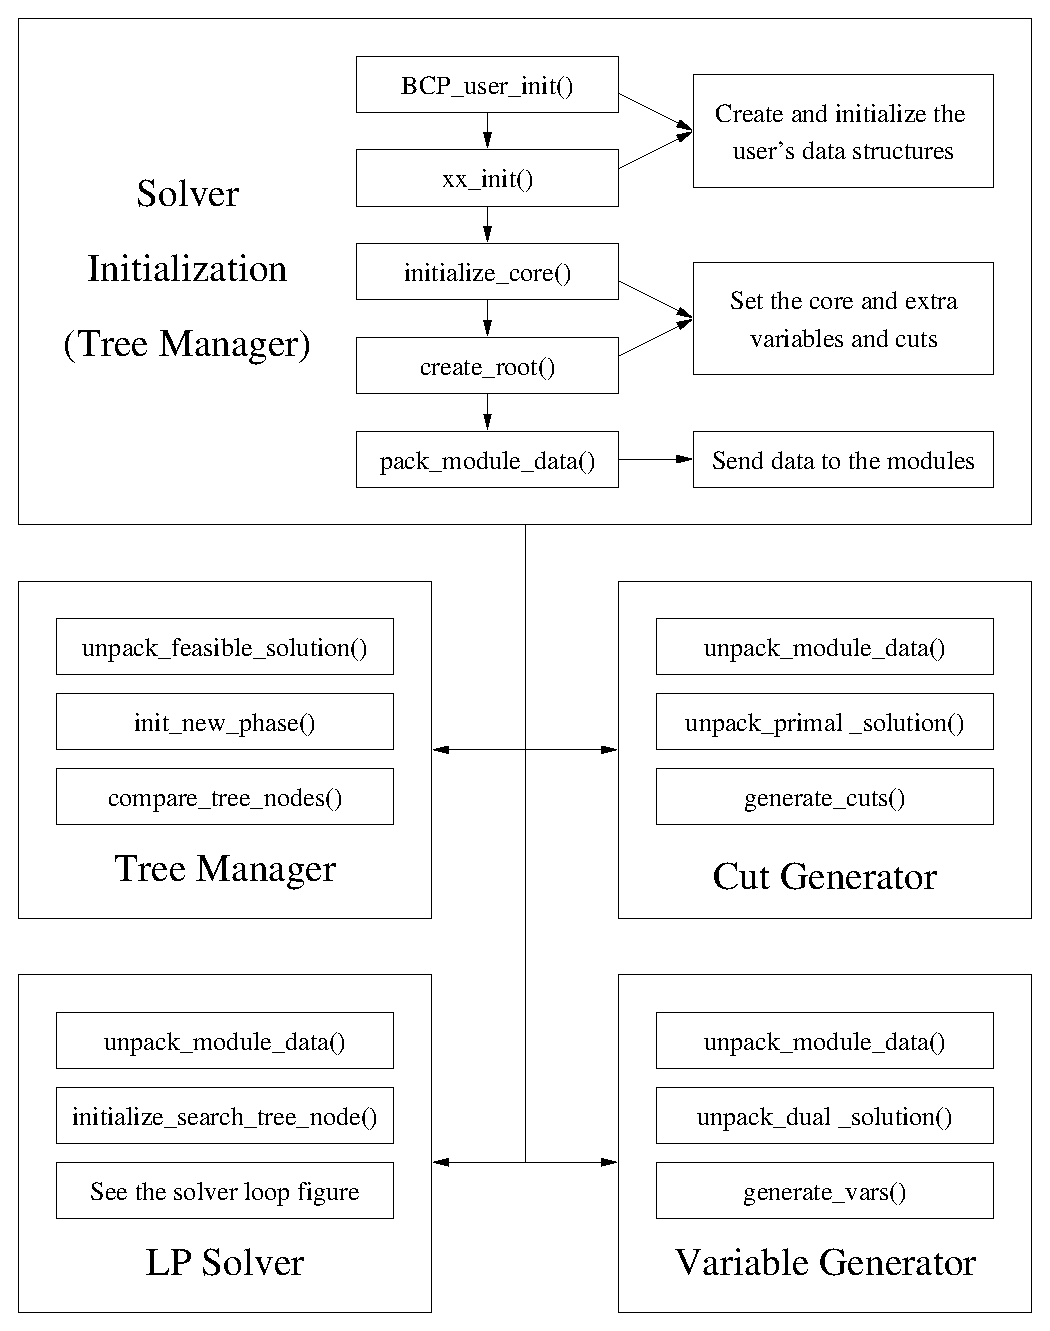
\includegraphics[scale=0.75]{flow-init.eps}
\end{center}
\caption{\label{dev:initmodule} Solver initialization and algorithm overview}
\end{figure}

\begin{figure}
\begin{center}
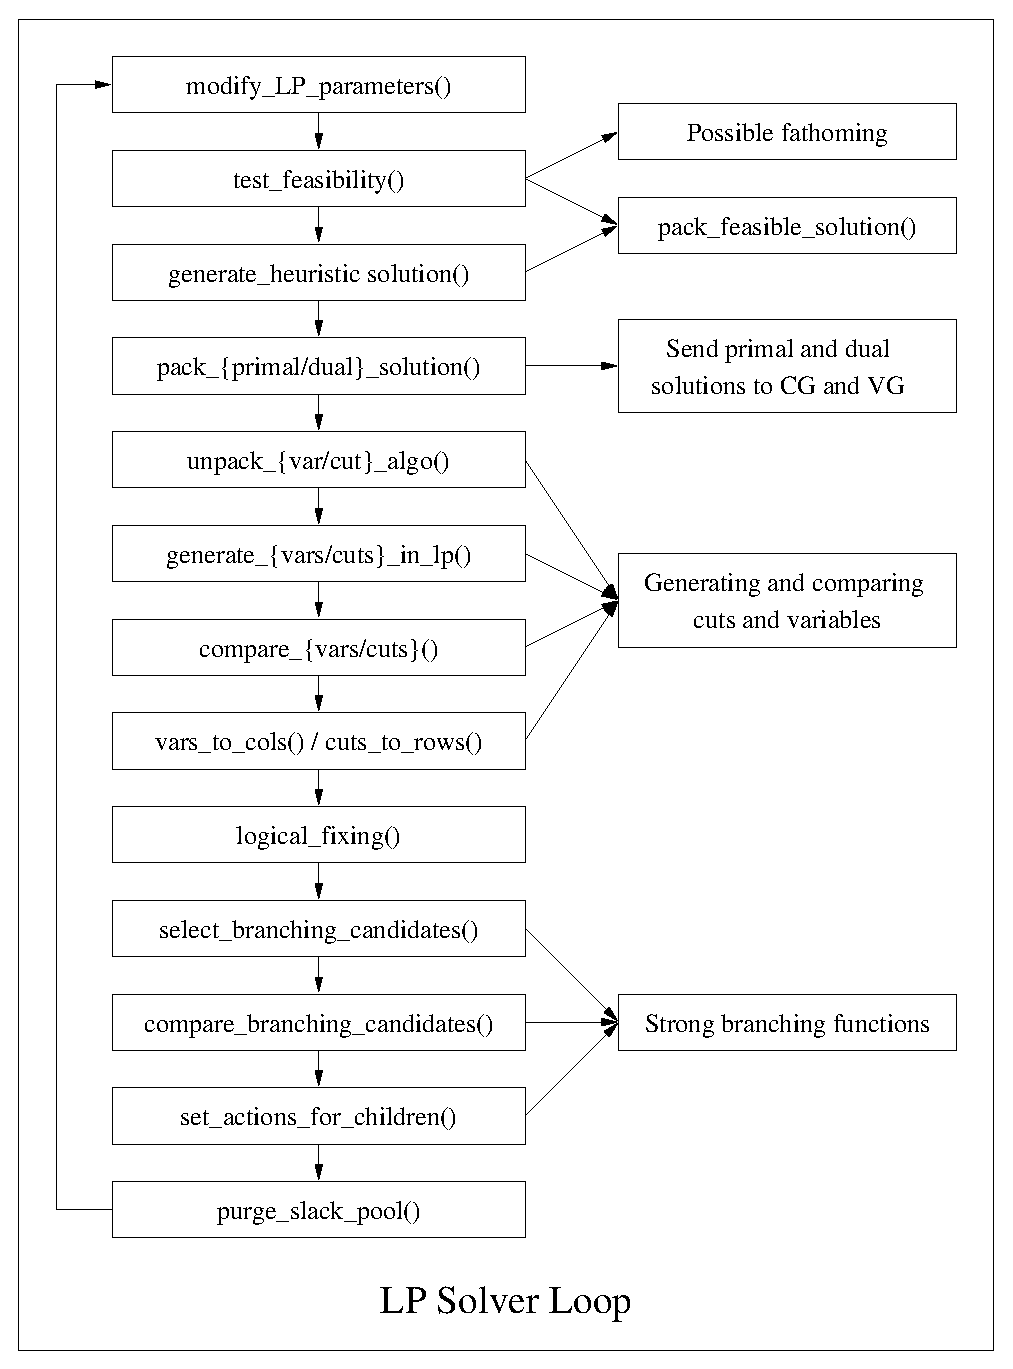
\includegraphics[scale=0.75]{flow-lploop.eps}
\end{center}
\caption{\label{dev:lploop}LP solver loop}
\end{figure}

\subsection{Fathoming procedure}

Fathoming, which is very simple
in a regular branch and cut algorithm is much more involved when
pricing is present. The reason is that introducing new columns can
push the lower bound below the global upper bound or can restore
feasibility if the LP relaxation was found infeasible. If a true
optimal solution is desired in a BCP algorithm, then a search tree
node can be fathomed if and only if there are no columns that can
restore feasibility and there is no column with negative reduced cost.
Of these two conditions the first one is the ``worse''. Almost always
there are variables that can be introduced to restore feasibility, but
usually that pushes the lower bound too high. However, we {\em must}
restore feasibility, because there can be columns with negative
reduced cost afterwards that could bring down the objective value. On
the other hand, when fathoming would happen because of too high lower
bound, all we got to look for are columns with negative reduced cost.
Frequently none are found (especially if the global upper bound is
really good) so the node can really be fathomed. For this reason it is
recommended that users wanting to generate variables on the fly set up
their model in a way that ensures primal feasibility at all times.
(Not to mention that then she doesn't have to override the feasibility
restoration methods.)

For each search tree node \BB\ maintains a state, that is, whether there are
indexed or algorithmic variables not in the formulation. Furthermore, for
indexed variables \BB\ can maintain a list about which ones have been
permanently priced out (excluded from any solution in the subtree). To utilize
this ability of \BB, only two very simple methods must be overridden:
\code{next\_indexed\_var()} and \code{create\_indexed\_var()}. The first
method is 
used to enumerate the indices of the indexed variables one by one, the second
method is used to actually create the indexed variables.

Now if fathoming would happen because the lower bound exceeds the upper bound
then, if \BB\ is instructed to maintain the above mentioned list, first the
not-yet-priced-out indexed variables are tested then the 
\code{generate\_vars\_in\_lp()} method is invoked for finding algorithmic
variables with negative reduced cost. 

If fathoming would happen because of infeasibility then again first the
indexed variables tested whether any of them destroys the proof of
infeasibility (i.e., whether it has a negative inner product with the
specified dual ray) then the \code{restore\_feasibility()} method is invoked so
that the user can test the algorithmic variables.

\section{Details of the Interface}
\label{dev:user-derived}

As mentioned earlier in our overview of the class hierarchy (Section
\ref{dev:overview-hierarchy}), the user can modify the behavior of the
framework by overriding the default methods. To override the methods
in a particular module, she simply derives a new child class from the
corresponding \code{BCP\_xx\_user} base class and overrides the
appropriate methods. If not overridden, the default method will be
invoked by the framework. Whenever possible, methods have default
which will work for the most common problem settings. In some cases,
there are several default implementations from which the user can
choose by setting a parameter. Alternatively, these methods can
be invoked directly by the user as desired, allowing for the use of
different methods in different situations. In the remainder of this
section, we describe in more detail the virtual methods of the
interface classes. These descriptions are at a high level---for the
exact specification, see the HTML manual pages included with the
distribution \cite{HTML-manual}.

\subsection{The \code{USER\_initialize} class}
\label{dev:USER_initialize}

The user must communicate the existence of the objects she designed to
\BB. For example, for all processes she intends to use she must have
derived something from the \code{BCP\_xx\_user} classes. Since \BB\
contains the \code{main()} function there are two ways to achieve this.
The ``C'' style solution is to have a functions declared in \BB\ but
not defined. These functions must be defined by the user and return
pointers to objects defined by her. The disadvantage of this solution
is that the user has to define all of these functions, even if she
doesn't intend to create some type of objects. Furthermore, if there
are possible defaults she must indicate somehow to the calling
function that a default should be executed.

\BB\ employs a C++ style coding here. Only one function is declared that the
user must define, \code{BCP\_user\_init()}. This function must
return an object of a type she derived from \code{USER\_initialize} and
in which she overrode some methods. This way the user is forced to
define only one function, and she can choose the default behavior
(like initializing the LP engine class) by simply not overriding a
method.

When \BB\ will be converted into a library there will be no need for this
class. 

\begin{itemize}
\item \code{msgenv\_init()}: return the message passing environment to be used.
  The user probably doesn't want to override this method, as the default 
  \BB\ uses will be determined by the value of \code{COMM\_PROTOCOL} in the
  application Makefile.
\item \code{tm\_init()}: return the object the user has derived from 
  \code{BCP\_tm\_user}. Note that this method should also take care of reading
  the parameter file and the problem data and whatever initialization the user
  wants to do. The user {\em must} override this method, there {\em must} be a
  user derived tree manager class.
\item \code{lp\_init()}: return the object the user has derived from 
  \code{BCP\_lp\_user}. The user {\em must} override this method, there 
  {\em must} be a user derived LP class.
\item \code{cg\_init()} and \code{vg\_init()}: return the object the user has
  derived 
  from the classes \code{BCP\_cg\_user} and \code{BCP\_vg\_user}. The user
  must override these if and only if she wants to generate cuts / variables.
\end{itemize}

\subsection{The \code{BCP\_tm\_user} class}

\begin{itemize}
\item \code{pack\_module\_data()}: in this method the user must pack the data
  that will be needed to perform computations in other modules. By default
  this method is empty and it is very likely that the user wants to override
  it.

  Note that this method should be overridden if and only if the 
  \code{unpack\_module\_data()} methods of any other process is overridden.

\item \code{unpack\_feasible\_solution()}: unpack a solution that is feasible
  to 
  the problem. Not really necessary to override, it should only be done if the
  default generic solution (\code{BCP\_solution\_generic}) format is not good
  for 
  the user for some reason. That format contains the description and value of
  all variables that are at nonzero level in the solution. The user may have a
  much more compact and intuitive representation of the solution, in which
  case she would override this method.

  By default a \code{BCP\_solution\_generic} object is unpacked.

  Note that this method should be overridden if and only if the corresponding
  method, \code{pack\_feasible\_solution()} in the class \code{BCP\_lp\_user}
  is 
  overridden.
  
\item \code{(un)pack\_warmstart()}: (un)pack warmstarting information for a
  search tree node. The user probably doesn't want to override this method, as
  it should correspond to the LP solver selected. The default, just like for
  the LP engine, will be determined by the defined \code{COIN\_USE\_XXX} value.

\item \code{(un)pack\_var\_algo()}: (un)pack an algorithmic variable. By
  default this method throws an exception since if it is invoked then the user
  must have generated an algorithmic variable in which case she must override
  this method.

\item \code{(un)pack\_cut\_algo()}: (un)pack an algorithmic cut. By
  default this method throws an exception since if it is invoked then the user
  must have generated an algorithmic cut in which case she must override
  this method.

\item \code{initialize\_core()} and \code{create\_root()}: the first of these
  two 
  methods sets up the core of the problem (see Section \ref{variables-cuts})
  while the second specifies what extra cuts and variables should be present
  in the root node. By default the first method creates an empty core and the
  second method does not list any extra objects. Therefore to get something
  into the root node the user must override at least one of them.
  
\item \code{init\_new\_phase()}: perform any necessary initialization before a
  new phase starts in the algorithm. Nothing is done as default. If the user
  does not do any pricing then the it is probably fine.  Otherwise (since the
  column generation strategy must be specified in this method, too) the user
  must override it.
  
\item \code{compare\_tree\_nodes()}: compare two search tree nodes. Return true
  if the first node should be processed before the second one. The default
  behavior is controlled by the \code{TreeSearchStrategy} parameter which is
  set to \code{BCP\_BestFirstSearch} by default. 

\end{itemize}

\subsection{The \code{BCP\_lp\_user} class}

This is by far the most complex class. 
\begin{itemize}
\item \code{unpack\_module\_data()}: unpack the data packed for this process in
  the TM by the \code{pack\_module\_data()} method. By default
  this method is empty and it is very likely that the user wants to override
  it.

  Note that if this method is overridden then the TM's
  \code{pack\_module\_data()} method must be overridden, too.

\item \code{(un)pack\_warmstart()}: (un)pack warmstarting information for a
  search tree node. The user probably doesn't want to override this method, as
  it should correspond to the LP solver selected. The default, just like for
  the LP engine, will be determined by the defined \code{COIN\_USE\_XXX} value.

\item \code{(un)pack\_var\_algo()}: (un)pack an algorithmic variable. By
  default this method throws an exception since if it is invoked then the user
  must have generated an algorithmic variable in which case she must override
  this method.

\item \code{(un)pack\_cut\_algo()}: (un)pack an algorithmic cut. By
  default this method throws an exception since if it is invoked then the user
  must have generated an algorithmic cut in which case she must override
  this method.
  
\item \code{initialize\_solver\_interface()}: return the LP engine. The user
  probably doesn't want to override this method as the default \BB\ uses will
  be determined by the defined \code{COIN\_USE\_XXX} value. However, it's
  possible that the user wants to define more than one LP solver and choose
  one based on a parameter.  In this case she needs to override this method.
  In this case she should also override the \code{(un)pack\_warmstart()}
  methods 
  in the TM and LP user classes as well.

\item \code{initialize\_new\_search\_tree\_node()}: do some preprocessing
  (e.g., 
  logical tightening of bounds on variables and/or constraints) on the
  search tree node before it gets processed. By default this method is empty.
  A good candidate for overriding in column generation methods, since there
  branching information usually encodes some logic, thus implying significant
  tightening.

\item \code{modify\_lp\_parameters()}: a chance to modify the parameters of the
  LP engine. By default this method is empty. Those experimenting with using
  different parameters in ``regular'' LP optimization and LP optimization in
  strong branching will want to override it.

\item \code{test\_feasibility()}: test whether the LP solution is feasible for
  the whole problem. If it is so then return a \code{BCP\_solution} object.
  The default just tests whether all integrality requirements are met.
  (Actually there are several default options but they differ in their speed
  only by exploiting special knowledge, e.g., knowing that all variable must
  be binary.) If the user has her own representation of the solution she
  definitely wants to override it (the default method creates a 
  \code{BCP\_solution\_generic} object). Also, she must override it if cuts are
  being generated as \BB\ has no way of knowing whether the not yet added cuts
  are all satisfied.

\item \code{generate\_heuristic\_solution()}: try to come up with a good
  solution 
  from the given LP solution. By default this method is empty. If the user has
  a quick heuristic it's worth to add it here since a good solution can
  drastically cut the size of the search tree. 

\item \code{pack\_feasible\_solution()}: the pair of
  \code{unpack\_feasible\_solution()} in the tree manager. Override neither or
  both. The default tries to treat and pack the solution argument as a 
  \code{BCP\_solution\_generic} object and throws an exception if it is not
  such a 
  solution. 
  
\item \code{pack\_primal\_solution()}: pack the information to be sent to the
  cut 
  generator (this is usually the primal solution). The default method packs a
  selected set of variables along with their values. The selection is
  parameter driven, it can be everything, the nonzeros, the fractional values,
  etc. Override neither or both of this method and its pair, 
  \code{unpack\_primal\_solution()} in the cut generator. There is no reason to
  override it if no cut generator processes are started.

\item \code{pack\_dual\_solution()}: pack the information to be sent to the
  variable generator (this is usually the dual solution). The default method
  packs a selected set of cuts along with their dual values. The selection is
  parameter driven, it can be everything, the nonzeros, the fractional values,
  etc. Override neither or both of this method and its pair, 
  \code{unpack\_dual\_solution()} in the variable generator. There is no reason
  to override it if no variable generator processes are started.

\item \code{display\_lp\_solution()}: display the result of most recent LP
  optimization. This method is invoked every time an LP relaxation is
  optimized and the user can display (or not display) it. By default the
  solution is displayed if the verbosity of \BB\ is high enough.

  This method exists mainly for debugging purposes. Few people would ever want
  to see all LP solutions. It's unlikely anyone would override this method.

\item \code{next\_indexed\_var()} and \code{create\_indexed\_var()}:
  methods used if \BB\ is to maintain the list of indexed variables that are
  permanently priced out. The first method returns the
  user index of the variable whose index is the next one after the argument
  while the second method creates an indexed variable (and the corresponding
  column) given the index.
  By default they all throw exceptions. The user must
  override them if they are to be used.

\item \code{restore\_feasibility()}:
  These methods are invoked before fathoming a search tree node that has
  been found infeasible. If \BB\ maintains the list of indexed variables that
  are permanently priced out then by the time this method is invoked every
  indexed variable is tested whether it can destroy the proof of
  infeasibility and the user should look only for algorithmic variables.
  Otherwise (i.e., if \BB\ does not maintain the list) it is up to the user to
  check both indexed and algorithmic variables whether they ``cut off'' the
  dual rays. 

\item \code{cuts\_to\_rows()}: create the corresponding rows for a set of cuts
  with 
  respect to the currently active variables. By default this method throws an
  exception (should not be called if not written). It must be overridden if
  cuts are generated.

\item \code{vars\_to\_cols()}: create the corresponding columns for a set of
  variables with respect to the currently active cuts. By default this
  method throws an exception (should not be called if not written). 
  It must be overridden if variables are generated.

\item \code{generate\_cuts\_in\_lp()}: generate cuts within the LP process.
  Sometimes too much information 
  would need to be transmitted for cut generation (e.g., the full tableau
  for Gomory cuts) or the cut generation is so fast that transmitting the
  info would take longer than generating the cuts. In such cases it might
  better to generate the cuts locally. This routine provides the opportunity.
  By default this method is empty (will be interfaced with Cgl).

\item \code{generate\_vars\_in\_lp()}: generate variables within the LP
  process. 
  Sometimes too much information 
  would need to be transmitted for variable generation or the variable
  generation is so fast that transmitting the info would take longer than
  generating the variables. In such cases it might be better to generate
  the variables locally. This routine provides the opportunity. By default
  this method is empty.

\item \code{compare\_cuts()}: compare two generated cuts. Cuts are generated in
  different iterations, 
  they come from the Cut Pool, etc. There is a very real possibility that
  the LP process receives several cuts that are either identical or one
  of them is better then another (cuts off everything the other cuts
  off). This routine is used to decide which one to keep if not both. By 
  default both cuts are kept. The user should override this method only if
  there is a significant chance that cuts will be regenerated.

\item \code{compare\_vars()}: compare two generated variables. Variables are
  generated in different 
  iterations, they come from the Variable Pool, etc. There is a very real
  possibility that the LP process receives several variables that are
  either identical or one of them is better then another (e.g., almost
  identical but has much lower reduced cost). This routine is used to
  decide which one to keep if not both. By 
  default both variables are kept. The user should override this method only
  if there is a significant chance that variables will be regenerated.

\item \code{logical\_fixing()}: this method provides an opportunity for the
  user 
  to tighten the bounds of variables. The method is invoked after reduced cost
  fixing. By default this method is empty. For many problems there are
  possibilities for tightening the bounds based on logical inferences. The
  user should explore this.

\item \code{select\_branching\_candidates()}: decide whether to branch or not
  and 
  select a set of branching candidates if branching is decided upon.
  The return value of the method indicates what should be done: branching,
  continuing with the same node or abandoning the node completely. The default
  implementation branches if there are no cuts or variables waiting to be
  added to the formulation. In that case it selects variables for strong
  branching. A good branching rule can really speed up computation. It's
  probably worth to override this method and experiment.

\item \code{compare\_branching\_objects()}: decide which one of two
  candidates should be selected for actual branching. The default
  implementation looks at the presolved objective values in the children and
  makes a decision based on those (the decision is parameter controlled).
  Probably the user is best off leaving this method alone.

\item \code{set\_actions\_for\_children()}: decide what to do with the children
  of the selected branching object. By default the possibility of diving is
  explored and then all or all but one (in case of diving) children are sent
  back to the tree manager. Probably the user is best off leaving this method
  alone. 

\item \code{purge\_slack\_pool()}: selectively purge the list of slack cuts.
  When a cut becomes ineffective and is eventually purged from the LP
  formulation it is moved into a slack pool. The user might
  consider these cuts later for branching. This function enables the user
  to purge any cut from the slack pool (those she wouldn't branch on
  anyway). Of course, the user is not restricted to these cuts when
  branching, this is only there to help to collect slack cuts. There are
  several default. The user probably doesn't want to override this method.

\end{itemize}

\subsection{The \code{BCP\_cg\_user} class}
This class is extremely simple. All it does is that it receives primal
solutions and generates cuts from them. If there is no separate cut generator
process the user doesn't need to derive a class from this one.

\begin{itemize}
\item \code{unpack\_module\_data()}: unpack the data packed for this process in
  the TM by the \code{pack\_module\_data()} method. By default
  this method is empty and it is very likely that the user wants to override
  it.

  Note that if this method is overridden then the TM's
  \code{pack\_module\_data()} method must be overridden, too.

\item \code{unpack\_primal\_solution()}: unpack the information sent from 
  the LP (this is usually the primal solution). The default method unpacks a
  set of variables along with their values. See the 
  \code{pack\_primal\_solution()} of the LP process.
  Override neither or both of this and that method.

\item \code{generate\_cuts()}: do the actual cut generation. By default this
  method is empty. The user better override it otherwise why have a separate
  CG process?

\item \code{unpack\_var\_algo()}: unpack an algorithmic variable. By
  default this method throws an exception since if it is invoked then the user
  must have generated an algorithmic variable in which case she must override
  this method. Note that in the cut generator there is no need to pack
  algorithmic variables. They are only received with the primal solution.

\item \code{pack\_cut\_algo()}: pack an algorithmic cut. By
  default this method throws an exception since if it is invoked then the user
  must have generated an algorithmic cut in which case she must override
  this method. Note that in the cut generator there is no need to unpack
  algorithmic cuts. They are only sent out to the LP process.


\end{itemize}

\subsection{The \code{BCP\_vg\_user} class}
This class is extremely simple. All it does is that it receives dual
solutions and generates variables from them. If there is no separate variable
generator process the user doesn't need to derive a class from this one.

\begin{itemize}
\item \code{unpack\_module\_data()}: unpack the data packed for this process in
  the TM by the \code{pack\_module\_data()} method. By default
  this method is empty and it is very likely that the user wants to override
  it.

  Note that if this method is overridden then the TM's
  \code{pack\_module\_data()} method must be overridden, too.

\item \code{unpack\_primal\_solution()}: unpack the information sent from 
  the LP (this is usually the dual solution). The default method unpacks a
  set of cuts along with their values. See the 
  \code{pack\_dual\_solution()} of the LP process.
  Override neither or both of this and that method.

\item \code{generate\_vars()}: do the actual variable generation. By default
  this 
  method is empty. The user better override it otherwise why have a separate
  VG process?

\item \code{pack\_var\_algo()}: pack an algorithmic variable. By
  default this method throws an exception since if it is invoked then the user
  must have generated an algorithmic variable in which case she must override
  this method. Note that in the variable generator there is no need to unpack
  algorithmic variables. They are only sent out to the LP process.

\item \code{unpack\_cut\_algo()}: unpack an algorithmic cut. By
  default this method throws an exception since if it is invoked then the user
  must have generated an algorithmic cut in which case she must override
  this method. Note that in the variable generator there is no need to pack
  algorithmic cut. They are only received with the dual solution.

\end{itemize}

\section{Deriving Problem-specific Classes}

In this section, we give a rough explanation of the design decisions
that have to be made and under what conditions the user needs to
derive certain types of classes and override certain methods.

\subsection{Generating cuts}

In some cases, such as in pure branch and bound or branch and price,
the user will not need to generate cutting planes dynamically, but for
most applications, dynamic cut generation is critical to the
efficiency of the algorithm. Assuming that the user has chosen to
perform dynamic cut generation, he must decide between the two
different types of cuts that can be dynamically generated---indexed,
and algorithmic. As we have already discussed, there is no theoretical
difference between these two types, but indexed cuts are more memory
efficient since they do not have to be represented by a (possibly)
bulky, abstract data structure. If it is possible to implement a
particular class of cuts using an indexing scheme, this should
generally be done. However, keep in mind that most classes of cuts
cannot be implemented using indexing simply because they are too
large to accomodate a workable indexing scheme.

For each class of cuts that the user wants to implement as an
algorithmic class, it will be necessary to derive a new C++ class from
\code{BCP\_cut\_algo} as a container for the data needed to construct
the cut. In addition, the user needs to modify the 
\code{pack\_cut\_algo()} and \code{unpack\_cut\_algo()} methods in the
appropriate \code{BCP\_xx\_user} classes. For indexed and core cuts, it
is not necessary to derive a new class or implement packing and
unpacking algorithms since all these cuts have a common
representation.

With either algorithmic or indexed cuts, the user must also override
the \code{cuts\_to\_rows()} and \code{compare\_cuts()} methods in the
\code{BCP\_lp\_user class}. The former specifies how to realize a given
set of cuts as matrix rows with respect to the current set of
variables while the latter is a function which determines if two cut
objects actually represent the same cut. Of course, in addition, the
user must also override either the \code{generate\_cuts()} method of
the \code{BCP\_cg\_user} class or the \code{generate\_cuts\_in\_lp()}
method of the \code{BCP\_lp\_user} class. The choice of whether to
generate cuts in a separate cut generator or simply as part of the LP
loop depends on the problem setting. In problems where generating cuts
is relatively quick and the LP solver will be sitting idle waiting for
the cut generator to return the cuts, it is easiest to simply generate
them in the LP module itself. If cut generation is lengthy or requires
large amounts of memory, then it is better to generate them in a
separate generator.

\subsection{Generating variables}

Generally speaking, dynamic variable generation (often called column
generation) is used less frequently than dynamic cut generation. If it
is possible to efficiently generate all variables explicitly in the
root node and there is enough memory to store them, this is generally
the best thing to do. This allows variables to be fixed by reduced
cost and nodes to be fathomed without expensive pricing (see the last
paragraph). However, sometimes this is either not possible or not
efficient because (1) there is not enough memory to store all of the
variables in the matrix at once, (2) it is expensive to generate the
variables, or (3) there is an efficient method of pricing large
subsets of variables at once. There may also be other scenarios
requiring variable generation.

In most ways, variable generation is similar to cut generation.
However, there are some significant differences. While generating cuts
helps tighten the formulation and increase the lower bound, generating
variables has the opposite effect. Therefore, one must be somewhat
careful about when variable generation takes place as it destroys
monotonicity of the objective function, upon which algorithmic
performance sometimes depends. In the last paragraph of this section,
we also address the issue of variable generation prior to fathoming a
search nodes, another important consideration.

As with cuts, the user must choose between the two different types of
variables---algorithmic, and indexed. Again, there is no theoretical
difference between these two types, but indexed variables are more
memory efficient than algorithmic variables. To utilize algorithmic
variables, the user should should derive a class or classes from 
\code{BCP\_var\_algo}, as with cuts. Also, the corresponding packing and
unpacking methods need to be modified appropriately. For indexed
variables, it is not necessary to derive a new class---the 
\code{BCP\_var\_indexed} class is provided for this purpose. In either case,
the user must also override the \code{vars\_to\_cols()} and 
\code{compare\_vars()} methods in the \code{BCP\_lp\_user class}. The former
specifies how to realize a given set of variable as matrix columns
with respect to the current set of cuts while the latter is a function
which determines if two variable objects actually represent the same variable.
As before, the user must also override either the 
\code{generate\_vars()} method of the \code{BCP\_vg\_user} class or the 
\code{generate\_vars\_in\_lp()} method of the \code{BCP\_lp\_user} class.

Our final consideration is that of fathoming. Before a node can be
properly fathomed in BCP, it is necessary to ensure that there are no
columns whose addition to the problem could reverse the conditions
necessary for fathoming the node in question, i.e., by either lowering
the objective function value back below the current upper bound or by
restoring feasibility. For indexed variables, the framework can
automatically keep track of which variables need to be priced out
before the search tree node can be fathomed. In order for this option
to be utilized, the user must provide the methods 
\code{next\_indexed\_var()} and \code{create\_indexed\_var()}. If this scheme
is not used, or the user is generating algorithmic variables, then the
user's variable generation method should expend whatever effort is
necessary to test whether there is a variable whose addition to the
problem would lower the objective function value, i.e., a variable
with negative reduced cost. Any such variable should be added to the
problem before fathoming. In addition, the user should either ensure
that all LP relaxation encountered are feasible (strongly encouraged)
or implement the \code{restore\_feasibility()} method. This method is when a
node would be fathomed because of infeasibility, and the user is supposed to
return new variables whose corresponding columns destroy the proof of
infeasibility (i.e., have negative inner product with the known dual rays).

\subsection{Setting the Core and Extra Object Lists}

Recall that the core cuts and variables are those that are never
removed from the problem. In some cases, significant savings can be
achieved by properly choosing the list of core and extra objects well.
To set the list of core objects, the user is required to override the
\code{initialize\_core()} methods in the \code{BCP\_tm\_user} class. There are
important differences between the strategy for setting the list of
core variables and that for setting the list of core cuts so we
address each of these topics separately in what follows.

In the current implementation, the main advantage of putting a
variable into the core is lower communication overhead and lower
overhead for node creation in the tree manager and node setup in the
LP module. Since variables in the core are present in every
relaxation, information about them does not have to be communicated
and stored along with each node description. Therefore, it is best to
put into the core any variable that has a high probability of having a
positive value in an optimal solution to the problem.

On the other hand, putting variables into the core that turn out not
to be important can cause the size of the matrices for the subproblems
to be bigger than necessary and can slow down the calaculation in
other ways. It is important to realize that, although putting
variables into the core does not prevent them from being fixed to zero
by reduced cost (and in essence removed from the calculation), they
must still be maintained as part of the matrix. In particular, when
cuts are put in row form to be added to the matrix, the coefficients
for these columns will have to be calculated, even though they are not
part of the calculation.

For cuts, some of the same factors are at work, but there is more at
stake, at least for simplex-based LP solvers. Although ineffective
cuts can similarly be removed from the problem by changing the right
hand side to $+\infty$ or $-\infty$, the number of rows that are
actually present in the matrix determines the size of the basis for
the simplex method. The size of the basis contributes significantly to
the overall running time of the simplex method. Hence, it is prudent
to allow removal of ineffective rows as soon as possible. One reason
for not allowing such removal is that it might be prohibitively
difficult or expensive to regenerate the row if it was ever needed
again. It might also be the case that some of the user's separation
algorithms depend on the fact that the solution already satisfies some
subset of inequalities. In this latter case, the most efficient way to
guarantee this might be to simply leave those cuts in the problem at
all times.

We have now seen the rationale for constructing the set of core
objects. The user can also optionally specify that a
designated subset of the extra cuts and variables (user indexed and/or
algorithmic) should be
initially present in the root, but not maintained as core objects.
These  variables and cuts are specified 
in the \code{create\_root()} method of the \code{BCP\_tm\_user}
class. The primary reason for designating these is that they are not
important enough to become core variables, but would be too expensive
to generate later, potentially over and over in various parts of the
tree. With respect to variables, it is usually best to include as many
of them as feasible in the root node. Provided that a good upper bound
exists, they will get priced out of the problem quickly if they are
not important. Also, their presence should not significantly slow down
simplex-based LP solvers. The same does not apply to cuts, however. It
is important to consider carefully the cuts that go into the base
since these will determine the starting size of the basis for
simplex-based LP solvers.

\subsection{Branching}

Next to effective cut and variables generation, strong branching is
the function most critical to the efficiency of BCP. Fortunately, the
framework takes care of most of the details. Furthermore, the defaults
should work fine in most cases. For instance, one of the built-in
defaults is to branch on the variable furthest from being integral
(closest to .5 for 0-1 problems. This is an often-used method that
will work fine for starting out. To implement his own branching
scheme, the user has only to implement two functions in the
{BCP\_lp\_user} class---\code{select\_branching\_candidates()} and 
\code{compare\_branching\_candidates()}. Based on knowledge of the problem's
structure, the user must decide which objects (cuts and/or variables)
to branch on. Unfortunately, there are not many rules of thumb here.
The only way to find out what works best in a particular problem
setting is trial and error.

\subsection{Summary and Optional Methodss}

In this subsection a summarized reference is provided for the classes and
subroutines that need to be considered based on various design decisions. For
each decision the methods to be implemented is listed. Optional methods not
discussed in this chapter are also included. For more on those methods, please
see the HTML documentation.

% Some magic with setting the spacing for these descriptions
\begin{description}
  \setlength{\itemsep}{2.5ex}

\item[Perform cut generation]\ \\
  \vspace{-4ex}
  \begin{itemize}
    \setlength{\itemindent}{-4ex}
    \setlength{\itemsep}{-.5ex}
  \item Derive a class for each cut type from \code{BCP\_cut\_algo}.
  \item Override \code{generate\_cuts\_in\_lp()} in
    \code{BCP\_lp\_user} class to generate cuts directly in the LP module.
  \item Override \code{generate\_cuts()} in \code{BCP\_cg\_user} 
    to generate cuts in a separate cut generation module.
  \item Override \code{cuts\_to\_rows()} in \code{BCP\_lp\_user}.
  \item Override \code{compare\_cuts()} in \code{BCP\_lp\_user} class.
  \item Override \code{(un)pack\_cut\_algo()} in the appropriate 
\code{BCP\_xx\_user} classes.
  \end{itemize}

\item[Perform column generation]\ \\
  \vspace{-4ex}
  \begin{itemize}
    \setlength{\itemindent}{-4ex}
    \setlength{\itemsep}{-.5ex}
  \item Derive a class for each variable type from \code{BCP\_var\_algo}.
  \item Override \code{generate\_vars\_in\_lp()} in \code{BCP\_lp\_user} 
    to generate variables directly in the LP module.
  \item Override \code{generate\_vars()} in \code{BCP\_vg\_user} 
    to generate variables in a separate variable generation module.
  \item Override \code{vars\_to\_cols()} in \code{BCP\_lp\_user}.
  \item Override \code{compare\_vars()} in \code{BCP\_lp\_user}.
  \item Override \code{(un)pack\_var\_algo()} in the appropriate 
    \code{BCP\_xx\_user} classes.
  \item To use the built-in mechanism for tracking which indexed
    variables have been priced out, override \code{next\_indexed\_var()}
    and \code{create\_indexed\_var()} in \code{BCP\_lp\_user}.
  \item Ensure that all LP relaxations remain feasible or
    override \code{restore\_feasibility()} in \code{BCP\_lp\_user}.
  \end{itemize}

\item[Customize strong branching]\ \\
  \vspace{-4ex}
  \begin{itemize}
    \setlength{\itemindent}{-4ex}
    \setlength{\itemsep}{-.5ex}
  \item Override \code{select\_branching\_candidates()}, 
    \code{compare\_branching\_candidates()}
    and \code{set\_actions\_for\_children()} in \code{BCP\_lp\_user}.
  \end{itemize}

\item[Set the problem core.]\ \\
  \vspace{-4ex}
  \begin{itemize}
    \setlength{\itemindent}{-4ex}
    \setlength{\itemsep}{-.5ex}
  \item Override \code{initialize\_core()} in {BCP\_tm\_user}.
  \end{itemize}

\item[Create the root node.]\ \\
  \vspace{-4ex}
  \begin{itemize}
    \setlength{\itemindent}{-4ex}
    \setlength{\itemsep}{-.5ex}
  \item Override \code{create\_root()} in {BCP\_tm\_user}.
  \end{itemize}

\item[Modify the LP solver parameters.]\ \\
  \vspace{-4ex}
  \begin{itemize}
    \setlength{\itemindent}{-4ex}
    \setlength{\itemsep}{-.5ex}
  \item Override \code{modify\_lp\_parameters()} in \code{BCP\_lp\_user}.
  \end{itemize}

\item[Define data structure to store and send feasible solutions.]\ \\
  \vspace{-4ex}
  \begin{itemize}
    \setlength{\itemindent}{-4ex}
    \setlength{\itemsep}{-.5ex}
  \item Derive a new solution class from {BCP\_solution}.
  \item Override \code{(un)pack\_feasible\_solution()} in the classes 
    \code{BCP\_lp\_user} (packing) and \code{BCP\_tm\_user} (unpacking).
  \end{itemize}

\item[Define data structure to send LP solutions.]\ \\
  \vspace{-4ex}
  \begin{itemize}
    \setlength{\itemindent}{-4ex}
    \setlength{\itemsep}{-.5ex}
  \item Override \code{(un)pack\_\{primal,dual\}\_solution()}
    in the classes \code{BCP\_lp\_user} (packing) and 
    \code{BCP\_\{cg,vg\}\_user} (unpacking).
  \end{itemize}

\item[Use a primal heuristic to generate feasible solutions.]\ \\
  \vspace{-4ex}
  \begin{itemize}
    \setlength{\itemindent}{-4ex}
    \setlength{\itemsep}{-.5ex}
  \item Override \code{generate\_heuristic\_solution()} in 
    \code{BCP\_lp\_user}.
  \end{itemize}

\item[Send problem-specific data to the modules.]\ \\
  \vspace{-4ex}
  \begin{itemize}
    \setlength{\itemindent}{-4ex}
    \setlength{\itemsep}{-.5ex}
  \item Override \code{(un)pack\_module\_data()} in the appropriate 
    \code{BCP\_xx\_user} classes.
  \end{itemize}

\item[Display solutions in user-defined format.]\ \\
  \vspace{-4ex}
  \begin{itemize}
    \setlength{\itemindent}{-4ex}
    \setlength{\itemsep}{-.5ex}
  \item Override \code{display\_xx\_solution()} in \code{BCP\_lp\_user()} 
    and/or \code{display\_solution()} in \code{BCP\_tm\_user}.
  \end{itemize}

\item[Perform logical fixing of variables.]\ \\
  \vspace{-4ex}
  \begin{itemize}
    \setlength{\itemindent}{-4ex}
    \setlength{\itemsep}{-.5ex}
  \item Override \code{logical\_fixing()} in \code{BCP\_LP\_user}.
  \end{itemize}

\end{description}


\commentout{
Table \ref{summary-decisions} provides a summarized
reference for the classes and subroutines that need to be considered
based on various design decisions. This includes other optional
methods not discussed in this section. For more on those
methods, please see the HTML documentation.

\begin{longtable}{|p{2in}|p{3.65in}|}
\caption{Summary of Design Decisions \label{summary-decisions}} \\

\hline

{\bf Design Decision} & {\bf Implementation} \\ 

\hline 

Perform cut generation. & 

\begin{minipage}[t]{3.65in}

$\bullet$ Derive a class for each cut type from {\tt BCP\_cut\_algo}.

$\bullet$ Override {\tt generate\_cuts\_in\_lp()} in
{\tt BCP\_lp\_user} class to generate cuts directly in the LP module.

$\bullet$ Override {\tt generate\_cuts()} in {\tt BCP\_cg\_user} 
to generate cuts in a separate cut generation module.

$\bullet$ Override {\tt cuts\_to\_rows()} in {\tt BCP\_lp\_user}.

$\bullet$ Override {\tt compare\_cuts()} in {\tt BCP\_lp\_user} class.

$\bullet$ Override {\tt pack\_cut\_algo()} and {\tt unpack\_cut\_algo()} 
in the appropriate {\tt BCP\_xx\_user} classes.

\end{minipage}\\

\hline 

Perform column generation. & 

\begin{minipage}[t]{3.65in}

$\bullet$ Derive a class for each variable type from {\tt BCP\_var\_algo}.

$\bullet$ Override {\tt generate\_vars\_in\_lp()} in {\tt BCP\_lp\_user} 
to generate variables directly in the LP module.

$\bullet$ Override {\tt generate\_vars()} in {\tt BCP\_vg\_user} 
to generate variables in a separate variable generation module.

$\bullet$ Override {\tt vars\_to\_cols()} in {\tt BCP\_lp\_user}.

$\bullet$ Override {\tt compare\_vars()} in {\tt BCP\_lp\_user}.

$\bullet$ Override {\tt pack\_var\_algo()} and {\tt unpack\_var\_algo()} 
in the appropriate {\tt BCP\_xx\_user} classes.

$\bullet$ To use the built-in mechanism for tracking which indexed
variables have been priced out, override {\tt next\_indexed\_var()}
and {\tt create\_indexed\_var()} in {\tt BCP\_lp\_user}.

$\bullet$ Either ensure that all LP relaxations remain feasible or
override {\tt restore\_feasibility()} in {\tt BCP\_lp\_user}.

\end{minipage}\\

\hline

Customize strong branching & 

\begin{minipage}[t]{3.65in}

$\bullet$ Override {\tt select\_branching\_candidates()}, 
{\tt compare\_branching\_candidates()}, 
and/or {\tt set\_actions\_for\_children()} in {\tt BCP\_lp\_user}.

\end{minipage}\\

\hline

Set the problem core. & 

\begin{minipage}[t]{3.65in}
$\bullet$ Override {\tt initialize\_core()} in {BCP\_tm\_user}.
\end{minipage}\\

\hline

Create the root node. & 

\begin{minipage}[t]{3.65in}

$\bullet$ Override {\tt create\_root()} in {BCP\_tm\_user}.

\end{minipage}\\

\hline

Modify the LP solver parameters. & 

\begin{minipage}[t]{3.65in}

$\bullet$ Override {\tt modify\_lp\_parameters()} in {\tt BCP\_lp\_user}.

\end{minipage}\\

\hline

Define data structure to store and send feasible solutions. & 

\begin{minipage}[t]{3.65in}

$\bullet$ Derive a new solution class from {BCP\_solution}.

$\bullet$ Override {\tt pack\_feasible\_solution()} in {\tt BCP\_lp\_user} and
{\tt unpack\_feasible\_solution()} in {\tt BCP\_tm\_user}. 

\end{minipage}\\

\hline

Define data structure to send LP solutions. & 

\begin{minipage}[t]{3.65in}

$\bullet$ Override {\tt (un)pack\_\{primal,dual\}\_solution()}
in the appropriate {\tt BCP\_xx\_user} classes.

\end{minipage}\\

\hline

Use a primal heuristic to generate feasible solutions. & 

\begin{minipage}[t]{3.65in}

$\bullet$ Override {\tt generate\_heuristic\_solution()} in 
{\tt BCP\_lp\_user}.

\end{minipage}\\

\hline

Send problem-specific data to the modules.  & 

\begin{minipage}[t]{3.65in}

$\bullet$ Override {\tt (un)pack\_module\_data()} in the appropriate 
{\tt BCP\_xx\_user} classes.

\end{minipage}\\

\hline

Display solutions in user-de\-fi\-ned format. & 

\begin{minipage}[t]{3.65in}

$\bullet$ Override {\tt display\_xx\_solution()} in {\tt BCP\_lp\_user()} 
and/or {\tt display\_solution()} in {\tt BCP\_tm\_user}.

\end{minipage}\\

\hline

Perform logical fixing of variables. & 

\begin{minipage}[t]{3.65in}

$\bullet$ Override {\tt logical\_fixing()} in {\tt BCP\_LP\_user}.

\end{minipage}\\

\hline

\end{longtable}
}

\section{Internal Data Structures}

With few exceptions, the data structures used internally by 
\BB\ are undocumented and most users will not need to access them
directly. However, if such access is desired, a pointer to the main data
structure used by each of the modules can be obtained simply by calling
the method \code{getXxProblemPointer()} of the \code{BCP\_xx\_user} class where
\code{xx} is the appropriate module. This method will return a pointer to the
data structure for the appropriate module. Casual users are advised against
modifying \BB's internal data structures directly.

\section{Inter-process Communication}
\label{communication}
The implementation of \BB\ strives to shield the user from having to know
anything about communications protocols or the specifics of inter-process
communication. This is achieved by creating a \code{BCP\_buffer} object and
whenever user data needs to be passed from one process to another the user is
asked to pack the data into this buffer on the sending side and to unpack the
data from another buffer on the receiving side. Sending the data around and
receiving it is entirely internal to \BB. Note that data must be unpacked in
exactly the same order as it was packed, as data is read linearly into and out
of the message buffer. The easiest way to ensure this is done properly is to
simply copy the pack statements into the unpacking function and change the
function names.

\section{Debugging Your Application}

\subsection{The First Rule}

\BB\ has many built-in options to make debugging easier. The most
important one, however, is the following rule. {\bf It is easier to
debug the fully sequential version than the fully distributed
version}. Debugging parallel code is not terrible, but it is more
difficult to understand what is going on when you have to look at the
interaction of several different modules running as separate
processes. This means multiple debugging windows which have to be
closed and restarted each time the application is re-run. Since the difference
between compiling an application for serial and parallel execution is as
little as changing a definition in the Makefile it is trivial to first compile
a serial code, debug it and then compile for parallel execution.
Make sure to set the \code{USER\_OPT} flag to
``\code{-g}'' in the application Makefile.

\subsection{Debugging with PVM}
\label{debugging-PVM}
If you wish to venture into debugging your distributed application,
then you simply need to set the parameter \code{DebugXxProcesses}, where 
\code{Xx} is the name of the module you wish to debug, 
to the value ``1'' (representing true) in the parameter file. 
This will tell PVM to spawn the particular process or
processes in question under a debugger. What PVM actually does in this
case is to launch the script \code{\$PVM\_ROOT/lib/debugger}. You will
undoubtedly want to modify this script to launch your preferred
debugger in the manner you deem fit. If you have trouble with this,
please send e-mail to the mailing list (see Section \ref{resources}).

It's a little tricky to debug interacting parallel processes, but you
will quickly get the idea. The main difficulty is in that the order of
operations is difficult to control. Random interactions can occur when
processes run in parallel due to varying system loads, process
priorities, etc. Therefore, it may not always be possible to duplicate
errors. To force runs that you should be able to reproduce, make sure
to disable timeout during cut generation which is a major source of
randomness. Furthermore, 
run with only one active node allowed at a time. This will keep the tree
search from becoming random. These two steps should allow runs to be
reproduced. You still have to be careful, but this should make things easier.

\subsection{Using \code{Electric Fence}}

The make file is already set up for compiling applications using 
\code{Electric Fence}. Instead of just typing \code{make} type 
\code{make ebcps}. The executable name is the same as described
earlier, but with an ``e'' in front of it.

\subsection{Using \code{Purify}}

The make file is already set up for compiling applications using 
\code{Purify} on platforms where it is available. Make certain that the
\code{purify} 
command is in your path and Instead of just typing \code{make} type 
\code{make pbcps}. The executable name is the same as described
earlier, but with an ``p'' in front of it.

%\section{Checking the Validity of Cuts and Tracing the Optimal Path}
%\label{debugging}
%Sometimes the only evidence of a bug is the fact that the optimal
%solution to a particular problem is never found. This is usually
%caused by either (1) adding an invalid cut, or (2) performing an
%invalid branching. There are two options available for discovering
%such errors. The first is for checking the validity of added cuts.
%This checking must, of course, be done by the user, but \BB\ can
%facilitate such checking. To do this, the user must fill in the
%function \code{user\_check\_validity\_of\_cut()} (see Section). 
%THIS function is called every time a
%cut is passed from the cut generator to the LP and can function as an
%independent verifier. To do this, the user must pass (through her own
%data structures) a known feasible solution. Then for each cut passed
%into the function, the user can check whether the cut is satisfied
%by the feasible solution. If not, then there is a problem! Of course,
%the problem could also be with the checking routine. To see how this is
%done, check out the sample application file \code{Vrp/cg\_user.c}.
%After filling in this function, the user must recompile everything
%(including the libraries) after uncommenting the line in the make file
%that contains ``\code{BB\_DEFINES += -DCHECK\_CUT\_VALIDITY}.'' Type
%``\code{make clean\_all}'' and then ``\code{make}.''
%
%Tracing the optimal path can alert the user when the subproblem which
%admits a particular known feasible solution (at least
%according to the branching restrictions that have been imposed so far)
%is pruned. This could be due to an invalid branching. Note that this
%option currently only works for branching on binary variables. To use
%this facility, the user must fill in the function 
%\code{user\_send\_feas\_sol()} (see Section). 
%All that is required is to pass out an array
%of user indices that are in the feasible solution that you want to
%trace. Each time the subproblem which admits this feasible solution is
%branched on, the branch that continues to admit the solution is
%marked. When one of these marked subproblems is pruned, the user is
%notified.
%
%\section{Using the \code{Interactive Graph Drawing} Software}
%\label{IGD}
%The Interactive Graph Drawing (IGD) software package is included with
%\BB\ and \BB\ facilitates its use through interfaces with the
%package. The package, which is a Tcl/Tk application, is extremely
%useful for developing and debugging applications involving graph-based
%problems. Given display coordinates for each node in the graph, IGD
%can display support graphs corresponding to fractional solutions with or
%without edge weights and node labels and weights, as well as other
%information. Furthermore, the user can interactively modify the graph
%by, for instance, moving the nodes apart to ``disentangle'' the
%edges. The user can also interactively enter violated cuts through the
%IGD interface.
%
%To use IGD, you must have installed PVM since the drawing window runs
%as a separate application and communicates with the user's routines
%through message passing. To compile the graph drawing application,
%type ``\code{make dglib dg}'' in the \BB\ root directory. The user
%routines in the file \code{dg\_user.c} can be filled in, but it is not
%necessary to fill anything in for basic applications. 
%
%After compiling \code{dg}, the user must write some subroutines that
%communicate with \code{dg} and cause the graph to be drawn.
%Regrettably, this is currently a little more complicated than it needs
%to be and is not well documented. However, by looking at the sample
%application, it is relatively easy to see how it should be done. To
%enable graph drawing, put the line \code{do\_draw\_graph 1} into the
%parameter file or use the \code{-d} command line option.

%\section{Other Debugging Techniques}
%
%Another useful built-in function is MakeMPS, which will write the
%current LP relaxation to a file in MPS format. This file can then be
%read into the LP solver interactively or examined by hand for errors.
%Many times, CPLEX gives much more explicit error messages
%interactively than through the callable library. The form of the
%function is 
%\begin{verbatim}
%void MakeMPS(LPData *lp_data, int bc_index, int iter_num)
%\end{verbatim}
%The matrix is written to the file ``{\tt
%matrix.[bc\_index].[iter\_num].mps}'' where {\em bc\_index} is the
%usually passed as the index of the current subproblem and {\em
%iter\_num} is the current iteration number. These can, however, be any
%numbers the user chooses. If \BB\ is forced to abandon solution
%of an LP because the LP solver returns an error code, the current LP
%relaxation is automatically written to the file ``{\tt
%matrix.[bc\_index].[iter\_num].mps}'' where {\em bc\_index} is the
%index of the current subproblem and {\em iter\_num} is the current
%iteration number. MakeMPS can be called using breakpoint code to
%examine the status of the matrix at any point during execution.
%
%Logging is another useful feature. Logging the state of the search tree can
%help isolate some problems more easily. See Section \ref{tm_params}
%for the appropriate parameter settings to use logging.

%\section{Controlling Execution and Output}
%\label{output}
%Calling \BB\ with no arguments simply lists all command-line options.
%Most of the common parameters can be set on the command line. Usually
%it is easier to use a parameter file. To invoke \BB\ with a parameter
%file type ``\code{master -f filename ...}'' where filename is the name
%of the parameter file. The format of the file is explained in Section
%\ref{parameter_file}. 
%
%The output level can be controlled through the use of the verbosity
%parameter. Setting this parameter at different levels will cause
%different progress messages to be printed out. Level 0 only prints out
%the introductory and solution summary messages, along with status
%messages every 10 minutes. Level 1 prints out a message every time a
%new node is created. Level 3 prints out messages describing each
%iteration of the solution process. Levels beyond 3 print out even more
%detailed information.

%There are also two possible graphical interfaces. For graph-based
%problems, the Interactive Graph Drawing Software allows visual display
%of fractional solutions, as well as feasible and optimal solutions
%discovered during the solution process. For all types of problems,
%VBCTOOL creates a visual picture of the branch and cut tree, either
%in real time as the solution process evolves or as an emulation from a
%file created by
%\BB. See Section \ref{tm_params} for information on how to use VBCTOOL
%with SYMPHONY. Binaries for VBCTOOL can be obtained at \\ 
%\code{\htmladdnormallink
%{http://www.informatik.uni-koeln.de/ls\_juenger/projects/vbctool.html}
%{http://www.informatik.uni-koeln.de/ls\_juenger/projects/vbctool.html}}.


%\subsection{Other Resources}
%\label{resources}
%There is a \BB\ user's list serve for posting questions/comments.
%To subscribe, send ``\code{subscribe symphony-users}'' to
%\code{\htmladdnormallink{majordomo@branchandcut.org}
%{mailto:majordomo@branchandcut.org}}. There is also a Web site for
%\htmladdnormallink{SYMPHONY}{http://branchandcut.org/SYMPHONY} 
%\begin{latexonly}
%at \code{http://branchandcut.org/SYMPHONY}
%\end{latexonly}.  
%Bug reports can be sent to \\
%\code{\htmladdnormallink{symphony-bugs@branchandcut.org}
%{mailto:symphony-bugs@branchandcut.org}}.


%To run in a distributed environment, the
%user must have installed {\em \htmladdnormallink{Parallel Virtual
%Machine}{http://www.ccs.ornl.gov/pvm/}} (PVM) software, available for
%free from Oak Ridge National Laboratories
%\begin{latexonly}
%at \code{http://www.ccs.ornl.gov/pvm/} 
%\end{latexonly}. 
%To run in a shared memory environment, the user must have installed an
%OpenMP compliant compiler. A cross-platform compiler called {\em
%Omni}, which uses \code{cc} or \code{gcc} as a back end, is available
%for free download
%\begin{latexonly}
%at \code{http://pdplab.trc.rwcp.or.jp/Omni}
%\end{latexonly}. 

%This section of the manual is concerned with the detailed
%specifications needed to develop an application using \BB. It is
%assumed that the user has already read the first part of the manual, which
%provides a high-level introduction to parallel branch, cut, and price
%and the overall design and use of \BB. 
%
%%%%%%%%%%%%%%%%%%%%%%%%%%%%%%%%%%%%%%%%%%%%%%%%%%%%%%%%%%%%%%%%%%%%%%%%%%%%%%


%\chapter{Sample Application: The Max Cut Problem}
%\label{sample}
%\input{man-maxcut}

\chapter{Sample Application: The MKC Problem}
\label{sample-mkc}
In this chapter we describe how the solver for the MKC problem were
implemented. This implementation is a sample for a column generation scheme;
no cut generation is done. Since this problem is not so well known, first we
will describe the problem setting then the implementation details.

%%%%%%%%%%%%%%%%%%%%%%%%%%%%%%%%%%%%%%%%%%%%%%%%%%%%%%%%%%%%%%%%%%%%%%%%%%%%%%%

\section{The MKC Problem}
\label{mkc:problem}

MKC stands for {\em Multiple Knapsack problem with Color constraints} as it is
derived by generalizing the multiple knapsack problem along two directions:
(i) adding assignment restrictions on items which can be assigned to a
knapsack, (ii) adding a new attribute (called ``color'') to the items and then
adding the associated ``color'' constraints which restrict the number of
distinct colors which can be assigned to a knapsack to two.

This problem is motivated by the surplus inventory matching problem in the
steel industry (\cite{KDTL}): before planning production, an attempt is made
to satisfy orders using leftover slabs from surplus inventory. The goal of
inventory matching is to maximize the total weight of the orders satisfied
from the leftover and to minimize the leftover weight of each slab used in the
matching. For each order we can identify a set of applicable slabs from the
surplus inventory.  These assignment restrictions are based on quality and
physical dimension considerations.  For any given order only slabs which are
of the same quality or better can be applied.  In addition, the thickness and
width requirements for each order need to be compatible with those of the slab
applicable.  These considerations restrict the number of applicable slabs for
each order. The color constraints place restrictions on the sets of orders
that can be matched to the same slab in the surplus inventory. Because of
processing considerations in the finishing line of a steel mill not all orders
assignable to a slab can be packed together on the slab. There is a route
associated with each order that specifies the set of process operations that
need to be applied in the finishing mill. Orders with different routes require
different process operations and are referred to as being of different types.
Slabs packed with different order types need to be cut before they are
processed in the finishing mill.  Since cutting slabs is expensive and often
the cutting machine is a bottleneck, strong constraints are posed in terms of
the number of allowed cuts per slab. The simplest and most commonly used
constraint used is to limit the number of required cuts to one; i.e., no more
that two order types are allowed on a slab.  In order to describe this
constraint formally we associate a unique {\em color} with each route code and
restrict the number of colors on a slab to be no more than two.  Notice that
this implies that we associate a color with each order based on its route
code.  This restricts the number of different order types on a slab to two and
the number of required cuts to be no more than one.

%%%%%%%%%%%%%%%%%%%%%%%%%%%%%%%%%%%%%%%%%%%%%%%%%%%%%%%%%%%%%%%%%%%%%%%%%%%%%%%

\section{Natural formulation for MKC}

This formulation has three sets of variables and four sets of constraints
modeling the various restrictions.
\begin{eqnarray}[r@{\eqsep}c@{\eqsep}lqql]
\multicolumn{3}{c}{
\max \sum_{i = 1}^{N}\sum_{j \in N^i} w^i x^i_j -
     \sum_{i = 1}^{N} (W_j - \sum_{j \in N^i} w^i x^i_j) z_j
} & \nonumber \\
\sum_{i \in N_j} w^i x^i_j & \le & W_j z_j & 1 \le j \le M \label{con-ks} \\
\sum_{j \in N^i} x^i_j     & \le & 1       & 1 \le i \le N \label{con-order} \\
\sum_{c \in C_j} y^c_j     & \le & 2       & 1 \le j \le M \label{con-col1} \\
x^i_j & \le & y^{c^i}_{j}  & 1 \le i \le N, ~j \in N_{i} \label{con-col2} \\
x^i_j & \in & \{0,1\}      & 1 \le i \le N, ~j \in N_{i} \nonumber \\
y^c_j & \in & \{0,1\}      & \forall c \in C_j, ~1 \le j \le M \nonumber \\
z_j   & \in & \{0,1\}      & 1 \le j \le M \nonumber 
\end{eqnarray}

\begin{table}[ht]
\caption{List of notations}
\begin{center}
\begin{tabular}{|l@{ : }l|} 
\hline
$N$ & Total number of orders.\\
$M$ & Total number of slabs. \\
$N^i$ & Set of slabs incident to order $i$. \\
$N_j$ & Set of orders incident to slab $j$. \\
$w^i$ & Weight of order $i$. \\
$W_j$ & Weight of slab $j$. \\ 
$C_j$ & Set of colors incident on slab $j$. \\
$c^i$ & The color of order $i$. \\
$x^i_j$ & 1 if order $i$ is assigned to slab $j$; 0 otherwise. \\
$y^c_j$ & 1 if orders of color $c$ obtain material from slab $j$; 0
otherwise.\\
$z_j$ & 1 if any order is incident to slab $j$; 0 otherwise. \\
\hline 
\end{tabular}
\end{center}
\end{table}

The total number of variables in this formulation is 
$$
\sum_{i=1}^{N} |N^i| + \sum_{j=1}^{M} |C_j| + M \quad=\quad 
\sum_{j=1}^{M} |N_j| + \sum_{j=1}^{M} |C_j| + M
$$
while the total number of constraints is $2\sum_{i=1}^{N} |N^i| + 2M + N$.

Constraints (\ref{con-ks}) specify that if a slab is used then the total
weight of the orders assigned to the slab cannot exceed the weight of the
slab; Constraint (\ref{con-order}) describes that each order will be made at
most once; while constraints (\ref{con-col1}) and (\ref{con-col2}) enforce the
coloring restriction.

Notice that the objective function is non-linear. However, since $z_j = 0$
forces $x^i_j$ to be zero for all $i \in N_j$ and $z_j = 1$ implies
$x^i_j z_j = x^i_j$, for all feasible solutions the objective function is
equivalent to 
$$
\sum_{i = 1}^{N}\sum_{j \in N^i} w^i x^i_j -
    \sum_{i = 1}^{N} ( W_j z_j - \sum_{j \in N^i} w^i x^i_j ) =
\sum_{i = 1}^{N}\sum_{j \in N^i} 2w^i x^i_j - \sum_{i = 1}^{N} W_j z_j 
$$.

The final observation is that the objective function just combines the two
stated goals (maximizing satisfied orders and minimizing wasted parts of
slabs) with equal weights. This may or may not be the best composite
objective, but this is how the creator of the application specified the
problem. Also, all that a different composite weight would change is the
multiplier $2$ for $w^i$ (the coefficient of $x^i_j$) and the multiplier $1$
for $W_j$ (the coefficient of $z_j$); nothing in the proposed algorithms would
need to be changed.

%%%%%%%%%%%%%%%%%%%%%%%%%%%%%%%%%%%%%%%%%%%%%%%%%%%%%%%%%%%%%%%%%%%%%%%%%%%%%%%

\section{A formulation suitable for column generation}

This new formulation has significantly more columns than the original
formulation, on the other hand it results in a well studied problem, the set
packing problem (\cite{NW}).

There are two types of constraints in this formulation. The first type
corresponds to the slabs in the problem, the second type to the orders. The
variables represent feasible production patterns, that is, variable $u$ has a
$1$ in the row corresponding to the slab the production pattern is to be made
of and $1$'s in the rows corresponding to the orders in the production
pattern. Each variable is a binary variable indicating whether that production
pattern is chosen in the solution or not. Let us introduce the following
notation:
\begin{itemize}
\item $P$ is the set of feasible production patterns;
\item $P_j$ is the set of set of feasible patterns manufacturable from slab
  $j$;
\item $P^i$ is the set of set of feasible patterns containing order $i$;
\item $R_k$ is the row (constraint) corresponding to the slab the production
  pattern corresponding to $u_k$ is made of; and
\item $R^k$ is the set of rows (constraints) corresponding to the orders in
  the production pattern corresponding to $u_k$.
\end{itemize}
Let the cost of variable $u_k$ be $\bar{c}_k = \sum_{i\in R^k} 2w^i - W_{R_k}$
and create the following set packing problem:
\begin{eqnarray}[rclqql]
\multicolumn{3}{l}{\max \sum_{k\in P} \bar{c}_k u_k} & \nonumber \\
\sum_{k\in P^i} u_k & \le & 1 & \forall 1 \le i \le N \\
\sum_{k\in P_j} u_k & \le & 1 & \forall 1 \le j \le M \\
\multicolumn{3}{l}{u_k\in\{0,1\}} & \forall k \in P \nonumber
\end{eqnarray}

It is very easy to see that there is a one to one correspondence between the
feasible solutions of this set packing problem and the feasible solutions of
the original formulation. Moreover, the construction of the $\bar c$ cost
vector ensures that the corresponding solutions have identical objective
values. Therefore optimizing this problem is the same as optimizing the
original formulation.

The obvious problem with this formulation is that the number of feasible
production patterns is enormous. 

\subsection{Generating columns with positive reduced costs}
To improve the solution evenly, for each slab we generate a production pattern
whose corresponding column has the highest reduced cost, i.e., the most
positive if there is one with positive reduced cost. Finding these columns is
again a set of optimization problems, since for a dual vector $\pi$ the
reduced cost of variable $u_k$ whose production pattern is made of slab $j$ is
simply
\begin{equation}
\bar{c}_k - \pi_j - \sum_{i\in R^k} \pi^i = 
\sum_{i\in R^k}2w^i - W_j - \pi_j - \sum_{i\in R^k} \pi^i =
- (W_j + \pi_j) + \sum_{i\in R^k} (2w^i - \pi^i)
\end{equation}
and we want to maximize this over the set of production patterns that can be
manufactured from slab $j$. For a fixed $j$ the first term is constant. The
feasible production patterns from slab $j$ are those that satisfy the capacity
and color constraints, thus this problem is equivalent to (using the notation
from the original formulation):
\begin{eqnarray}[rcl]
\multicolumn{3}{l}{\max\sum_j (2w^i - \pi_i) x^i_j} \\
\sum_i w^i x^i_j & \le & W_j \\
\sum_i y^{c(i)}_j & \le & 2 \\
\multicolumn{3}{l}{x^i_j \in \{0,1\}}
\end{eqnarray}
which is a knapsack problem with the side constraint that selected objects
must have no more than two different colors. Moreover, the constant term in
the reduced cost implies that we are only looking for production patterns
whose reduced cost exceeds $W_j + \pi_j$. Since solving the LP relaxation of
the knapsack problem (even with the side constraint) is rather simple, this
required lower bound on the reduced cost can be very helpful in quickly
concluding that there is no improving pattern for a particular slab.

\subsection{Upper bounding}

The previous subsection addresses the issue of how to solve the full LP
relaxation by iteratively solving smaller LP relaxations and generating
columns, but we need something more. We need to be able to derive an upper
bound on the optimal objective value of the full LP relaxation in every
iteration. There are two reasons for this. The first is that in a
Branch-and-Price algorithm we can fathom a search tree node if the upper bound
on the optimal objective value of the LP relaxation at the node is already
lower than the value of a currently known feasible solution. Since we may not
be able to solve the subproblems that generate the columns (after all, even
though the knapsack problem is considered relatively easy, it {\em is}
NP-complete) we still want to have an upper bound for fathoming purposes. The
second reason is that without an upper bound on the optimal value of the LP
relaxation of the full problem we couldn't tell how close we are to
optimality, we wouldn't have a proven gap.

Fortunately, upper bounding is very easy using Dantzig-Wolfe decomposition
\cite{dantzig-wolfe}. Since the sum of all variables in $P_i$ is not more than
$1$, the objective value of the LP relaxation cannot change more than the
highest reduced cost (or an upper bound on that value) as a result of changing
the values of the variables in $P_i$. To get an upper bound on the reduced
cost we can use the LP relaxation of the subproblem (the side constrained
knapsack problem) which is very easy to solve. Now adding all ``per slab''
upper bounds to the optimal objective value of the current LP relaxation
yields an upper bound on the optimum of the full LP relaxation.

\subsection{Finding integral feasible solutions}

Another advantage of the column generation based formulation is that it is
very easy to generate feasible solutions. In each iteration we considered the
fractional solution and started by including every variable above $0.5$ in the
solution. From the set of remaining fractional variables we exluded all that
intersected the already selected variables. Whatever remained afterwards was
always such a small set that we could solve the set packing problem on that
set by enumeration.

%%%%%%%%%%%%%%%%%%%%%%%%%%%%%%%%%%%%%%%%%%%%%%%%%%%%%%%%%%%%%%%%%%%%%%%%%%%%%%%

\section{Implementation details}

\subsection{Cuts, variables and solutions}
First of all, we did not have to worry about anything cut generation related,
since we were not generating cuts. Since the number of constraints is not too
great (number of orders + number of slabs) we decided to treat all of them as
core constraints, thus completely eliminating the need to bother about cuts.

For the variables first we had to decide which ones are going to be core
variables and which ones will be extra variables. Since we had no
reason to believe that any one particular pattern was more likely to be in
an optimal solution than some other pattern we decided not to have core
variables at all (this also simplified coding somewhat). Since the variables
are the feasible production patterns, they do not lend themselves to any
enumeration scheme, so we decided not to have indexed variables either.
Therefore all our variables are algorithmic ones. Actually, we had two kind of
algorithmic variables, one for the production patterns and another one for
branching, but we will discuss that latter in Section \ref{mkc:branching}. Both
types of variables are derived from \code{BCP\_var\_algo} and are defined in
\code{MKC\_var.hpp}.

We have defined our solution class for two reasons. First, all our pattern
variables are binary variables so there is no reason to include the value of
the non-zero ones. Second, there might be branching variables (not pattern
variables) that are at nonzero level as we go down in the tree, and we didn't
want to include those in a feasible solution. Still, if we wanted to, we could
have used a generic solution type. We just thought that using our own solution
type makes the code clearer. 

\subsection{Branching}
The problem with branching when generating columns is that we must be able to
generate columns after branching, too. In other words, every generated column
must conform to whatever branching decisions have been made to that point.
That means that branching on a regular variable is out of question. On one
side (when it is fixed to 1) we'd have great results, it would significantly
shrink the search space. However, on the other side (fixing the variable to 0)
the restriction is that we cannot regenerate that variable. But that variable
will almost always ``want to be regenerated'' (definitely immediately after
branching), since its reduced cost will make it attractive (after all, we have
forcibly moved it away from where it ended up in the LP-optimal solution). So
for our problem this would mean that after one branching we have to check the
optimal solution to the knapsack subproblem and if it is the forbidden
variable then we have to find the second best solution. After two branchings
we may have to find the third best solution, etc. This is impossible. 

Instead, the following logic is introduced. A branching object will specify
whether a particular order $O$ is manufactured from slab $S$ or not.

\subsection{Packing and unpacking}

Packing and unpacking of user objects is really straightforward. For example,
look at the \code{MKC\_var\_(un)pack()} functions. The packing function packs
the 
type of each variable and invokes the pack member of the variables while the
unpacking function unpacks the types and invokes the appropriate constructor. 

In general, when an object is packed it is simply torn down to built-in types
and those are packed. On the other side the date is unpacked in the same order
and the appropriate objects are constructed. In the following subsection we
will not mention the (un)packing member methods.

\subsection{MKC\_init}

This is the implementation of the intializer class. The TM initializer reads
in the problem and the parameters. Unfortunately this piece is rather
complicated since the problem is specified as an MPS file and we have to
extract order and slab information from it. The problem is loaded into the
\code{kss} member of the \code{MKC\_tm} class. See the \code{MKC\_knapsack.hpp}
file for data structures. Once the problem is read in a pointer to the 
\code{MKC\_tm} class is returned. The LP initializer just returns a pointer to
an empty \code{MKC\_lp} object.

\subsection{MKC\_tm}

There were only four methods (besides the (un)packing ones) we had to deal
with. Initializing the core consisted of simply specifying the core cuts as we
had no core variables (hence no core matrix). Since we had no core variables
we had to add some extra variable in creating the root. There are two options
for this, one is to add those variables that were read in from a file (maybe
as a result of a previous run), or we could generate columns for the all zero
dual solution (which is in some sense the optimal solution if we have no
variables...). Displaying the solution has the option to test the solution
that it really satisfies the original formulation (we have used this for
debugging purposes) and then the solution is printed in two different ways.
Finally, there will be only one phase and we will generate columns in it, so
we set this in the \code{init\_new\_phase()} method.

\subsection{MKC\_lp}







\chapter{Sample Application: The Maximum Cut Problem}
\label{sample-mcp}
In this cahpter, we describe the implementation of a sample
application---a solver for the maximum cut problem. This application
is a prototypical example of branch and cut, i.e., BCP with a fixed
set of variables. No column generation is used in this implementation.
This simplifies many of the basic tasks.

%%%%%%%%%%%%%%%%%%%%%%%%%%%%%%%%%%%%%%%%%%%%%%%%%%%%%%%%%%%%%%%%%%%%%%%%%%%%%%%

\section{The Max Cut Problem}
\label{MCP}

Given an undirected graph $G=(N,E)$ with edge weight function $\omega:
E \rightarrow {\rm \bf R}$, the Maximum Cut Problem (MCP) is that of
partitioning the nodes into two subsets in such a way that the total
weight of the edges in the cut separating the two sets is maximized.
This is a well-known problem---several branch and cut algorithms for
dense graphs have been presented in 
\cite{A:barahona-junger-reinelt,A:desimone-rinaldi}. In the following
description, we consider complete graphs only. For a complete graph
undirected graph with $n$ nodes, a linear relaxation of the integer
programming problem is givem by
\begin{eqnarray}
\min \;\; & c^Tx & \nonumber \\
{\rm s.t.} \;\;\; && \nonumber \\
& x_{ij}+x_{jk}+x_{ik} \le  2 & \;\;\;\forall (i,j,k) \in N^3 
\label{tri-0} \\
& x_{ij}-x_{jk}-x_{ik} \le  0 & \;\;\;\forall (i,j,k) \in N^3 
\label{tri-1} \\
& \hskip .51in 0 \le x_{ij} \le 1 & \;\;\;\forall (i,j) \in E \\
\end{eqnarray}
Here $x_{ij}$ takes value 1 if the edge $(i,j)$ appears in the cut, and 0
otherwise. Constraints (\ref{tri-0}) - (\ref{tri-1}) are called the
{\it triangle inequalities} and they define facets of the cut polytope
(see \cite{A:barahona-mahjoub:cut-polytope}).

Another set of inequalities, which is a superset of (\ref{tri-0}) -
(\ref{tri-1}), is the following. Let $C$ be a cycle and $F \subseteq
C$ with $|F|=2k+1$. Then
\begin{equation}
\sum_{e \in F} x_e - \sum_{e \in C\backslash F} x_e \le |F|-1 \label{c}
\end{equation}
is a valid inequality. This follows from the fact that the
intersection of a cycle and a cut has even cardinality. Note, that
although this set of inequalities include those in (\ref{tri-0}) -
(\ref{tri-1}), the polytope defined by these is the same, i.e., these
inequalities can be derived from those in (\ref{tri-0}) -
(\ref{tri-1}) (see \cite{A:barahona-mahjoub:cut-polytope}).

A polynomial time separation algorithm for this class of inequalities
has been given in \cite{A:barahona-mahjoub:cut-polytope}. 
However we use a faster heuristic as
follows. Let $\bar{x}$ be the fractional solution we want to separate
and define weights
\begin{equation}
w_e = c_e \cdot \max(\bar{x}_e, 1-\bar{x}_e).
\end{equation}
Then find a maximum weighted spanning tree $T$ with weights $w$. For
an edge $e \in T$, if $\bar{x}_e \ge 1-\bar{x}_e$ then the end-nodes
of $e$ should be on opposite sides of the cut---we give a label ``A''
to this edge. Otherwise, if $ \bar{x}_e < 1-\bar{x}_e$ then the
end-nodes should be on the same side of the cut, and we give the label
``B'' to this edge. Once every edge in $T$ has been labeled we have a
heuristic cut $K$. For each edge $e \notin T$, we add it to $T$ and
look at the cycle $C$ that is created. If $e \in K$, we test the
violation of an inequality (\ref{c}), where the set $F$ is given by
the A-edges. If $e \notin K$ the set $F$ is given by the A-edges and
the edge $e$. Although, as we noted above, inequalities (\ref{c}) are
implied by (\ref{tri-0}) - (\ref{tri-1}), we use (\ref{c}) because our
simple separation heuristic is faster than enumerating triangles.

\section{Implementation}

Because the size of the problems we can currently solve is small, we
can easily include all the edge variables explicitly. Hence, we do not
need to consider dynamiuc column generation. Hence, we do not need to
concern ourselves with the {\tt BCP\_vg\_user} class or the {\tt
BCP\_var\_algo} class. To simplify things further, we decided not to
use a separate cut generator either. This is usually a good approach
when cut generation is relatively inexpensive. It is also a good idea
during initial development since it makes debugging much easier.
Because we are not using a separate cut generator, we do not need to
consider the {\tt BCP\_cg\_user} class either.

As with virtually any BCP implementation, we will need to consider the
{\tt BCP\_tm\_user} and {\tt BCP\_lp\_user} classes. Also, because we
will be dynamically generating algorithmic cuts, we will need to
derive a new class to represent the cycle cuts (\ref{c}) from the
class {\tt BCP\_cut\_algo}. Finally, we will need to derive a new
class for describing the feasible solutions from {\tt BCP\_solution}.
In the remainder of the section, we provide a high-level description
of each of these classes. The reader is encouraged to look at the
source code and the HTML documentation for more detail. See Chapter
\ref{getting-started} for information on getting and examining the
source code and documentation.

\subsection{\tt MC\_tm}
\label{MC-tm}

This is the class derived from the {\tt BCP\_tm\_user} class. This
class is derived for the purpose of overriding a variety of functions
that we need to customize. These consist mainly of routiines that pass
data between the processes during parallel execution and the routines
for describing the problem core and root node. Below, we list each
function and describe how it was re-implemented.

\begin{itemize}

        \item {\tt unpack\_feasible\_solution()}: This subroutine
        exists to unpack the user-defined solution class described in
        Section \ref{MC-solution}. The corresponding {\tt
        pack\_feasible\_solution()} routine will be described in
        Section \ref{MC-lp}. Also, see Section \ref{MC-solution} for a
        description of how the feasible solutions are represented.
        
        \item {\tt pack\_module\_data()}: Here, we are packing the
        data that needs to be sent to the LP process. This consists of
        the number of nodes and a list of the edges in the graph. The
        corresponding {\tt unpack\_module\_data()} routines is
        described in Section \ref{MC-lp}.

        \item {\tt pack\_cut\_algo()}: Here, we pack the cycle cuts to
        be sent to the LP solver. The corresponding {\tt
        unpack\_cut\_algo()} routines is described in Section
        \ref{MC-lp}.

        \item {\tt unpack\_cut\_algo()}: Here, we unpack the cycle
        cuts that are received from the LP solver. The corresponding
        {\tt pack\_cut\_algo()} routines is described in Section
        \ref{MC-lp}.

        \item {\tt initialize\_core()}: Essentially for convenience
        and ease of implementation, we place all the variables in the
        core. This is possible since we are not using column
        generation, but may not be the most efficient method. None of
        the cuts are placed in the core since we don't have an
        inherently important subset that we know should never be
        removed from the problem.

        \item {\tt create\_root()}: To initialize the root node, we
        use some heuristics to generate an initial set of cycle cuts.
        However, as noted before, these are ``extra'' cuts and do not
        get put into the core. They may be removed later in the
        calculation. 

        \item {\tt display\_feasible\_solution()}: This routine is
        used essentially to display the solutions in a more
        ``user-friendly'' way, instead of simply as a list of variable
        indices and values. See Section \ref{MC-solution} for a
        description of how the feasible solutions are represented.

\end{itemize}

\subsection{\tt MC\_lp}
\label{MC-lp}

This is the class derived from the {\tt BCP\_lp\_user} class. Again, this
class is derived for the purpose of overriding a variety of functions
that we need to customize. These consist not only of routiines that pass
data between the processes, as before, but also routines for
generating cuts and performing strong branching. Below, we list each
function and describe how it was re-implemented.

\begin{itemize}

        \item {\tt unpack\_module\_data()}: Here, we unpack the data
        sent from the TM. This data is stored in a user-defined class
        called {\tt MC\_problem}.

        \item {\tt pack\_cut\_algo()}: Here, we pack the cycle cuts to
        be sent to the TM. The cuts are represented as a list of
        edges---first the edges in the set $F$, then the edges not in
        $F$. To contruct the corresponding valid inequality, we need
        only determine which edges variables are present in the
        relaxation. See the description of {\tt cuts\_to\_rows()} below.

        \item {\tt unpack\_cut\_algo()}: Here, we unpack the cycle
        cuts that are received from the TM along with the description
        of a subproblem.

        \item {\tt modify\_lp\_parameters()}: Here, we modify the LP
        parameters before solution of the relaxation commences.

        \item {\tt test\_feasibility()}: Because integrality of the
        solution is not enough to imply feasibility, we needed to
        override this method. If it is found that the solution is
        integral but not feasible, then cuts proving the infeasibility
        are easy to derive and are added to the LP relaxation,
        allowing the solution process to continue.

        \item {\tt pack\_feasible\_solution()}: Here, any feasible
        solutions that are found are packed and sent to the TM for
        storage. See Section \ref{MC-solution} for a description of
        how the feasible solutions are represented.

        \item {\tt cuts\_to\_rows()}: This subroutine generates the
        rows of the current LP relaxation corresponding to the cuts to
        be added. For cycle cuts, this consists simply of determining
        which of the edge variables that have a positive coefficient in
        the cycle cut, i.e., the variables corresponding to the edges
        of the corresponding cycle, are active in the current
        subproblem. For each variable corresponding to an edge that is
        in the cycle cut and also active in the subproblem, the
        corresponding matrix coefficient must be added to the
        row description.

        \item {\tt compare\_cuts()}: This routine simply compares two
        cuts and determines if they are the same cut. In the case of
        cycle cuts, this is straightforward.

        \item {\tt generate\_cut\_in\_lp()}: This is the subroutine
        that generates the cuts to be added to the relaxation. A
        description of the algorithm for generating the cycle cuts was
        given in Section \ref{MCP}.

        \item {\tt select\_branching\_candidates}: Here, we select the
        edges to be branched on. We branch basically on edges that are
        have high cost and are close to value .5.

\end{itemize}

\subsection{\tt MC\_solution}
\label{MC-solution}

Although feasible solutions to this problem consist of a set of edges,
they can be more compactly represented as simply a list of the nodes
contained in either shore of the cut. This user-defined class is used
for representing the solutions in this more compact, intuitive
fashion.

\subsection{\tt MC\_cycle\_cut}

This class was derived from {\tt BCP\_cut\_algo} to contain the
representation of the cycle cuts (\ref{c}). They are stored simply as
a list of edges in the cycle. The list is in two parts---first, the
edges in the set $F$ are listed and then those not in the set $F$. Of
course, the cardinality of the set $F$ has to be stored as well.

\subsection{Other Classes}

There are a number of other classes that we have defined to hold
data used during the solution process. Please see the HTML
documentation and the source code itself for a list of these. 




%\chapter{\BB\ Parameters}
%\label{params}
%\label{parameter_file}
The parameter file name is passed to \BB\ as the only command line
argument to the master process which is started by the user. Each line
of the parameter file contains either a comment or two words -- a
keyword and a value, separated by white space. If the first word
(sequence of non-white-space characters) on a line is not a keyword,
then the line is considered a comment line. Otherwise the parameter
corresponding to the keyword is set to the listed value. Usually the
keyword is the same as the parameter name in the source code. Here we
list the keywords, the type of value that should be given with the
keywords and the default value. A parameter corresponding to keyword
``K'' in process ``P'' can also be set by using the keyword ``P\_K''.

To make this list shorter, occasionally a comma separated list of parameters
is given if the meanings of those parameters are strongly
connected. For clarity, the constant name is sometimes given instead
of the numerical value for default settings and options. The
corresponding value is given in curly braces for convenience.

\subsection{Global parameters}
\begin{description}

\item[{\tt verbosity} -- integer (0).]
Sets the verbosity of all processes to the given value. In general,
the greater this number the more verbose each process is. Experiment
to find out what this means.

\item[{\tt random\_seed} -- integer (17).]
A random seed.

\item[{\tt granularity} -- double (1e-6).]
should be set to ``the minimum difference between two distinct
objective function values'' less the epsilon tolerance. E.g., if every
variable is integral and the objective coefficients are integral then
for any feasible solution the objective value is integer, so {\tt
granularity} could be correctly set to .99999.

\item[{\tt upper\_bound} -- double (none)].
The value of the best known upper bound.

\end{description}

\subsection{Master Process parameters}
\begin{description}

\item[{\tt M\_verbosity} -- integer (0).]

\item[{\tt M\_random\_seed} -- integer (17).]
A random seed just for the Master Process.

\item[{\tt upper\_bound} -- double (no upper bound).]
This parameter is used if the user wants to artificially impose an
upper bound (for instance if a solution of that value is already
known).

\label{upper_bound_estimate}
\item[{\tt upper\_bound\_estimate} -- double (no estimate).]
This parameter is used if the user wants to provide an estimate of the
optimal value which will help guide the search. This is used in
conjunction with the diving strategy \htmlref{\tt
BEST\_ESTIMATE}{diving_strategy}.

\item[{\tt tm\_exe, dg\_exe} -- strings (``tm'', ``dg'').]
The name of the executable files of the TM and DG processes. Note that
the TM executable name may have extensions that depend on the
configuration of the modules, but the default is always set to the
file name produced by the make file. If you change the name of the
treemanager executable from the default, you must set this parameter
to the new name.

\item[{\tt tm\_debug, dg\_debug} -- boolean (both {\tt FALSE}).]
Whether these processes should be started under a debugger or not (see
\ref{debugging-PVM} for more details on this).

\item[{\tt tm\_machine} -- string (empty string).]
On which processor of the virtual machine the TM should be run. Leaving this
parameter as an empty string means arbitrary selection.

\item[{\tt do\_draw\_graph} -- boolean ({\tt FALSE}).]
Whether to start up the DG process or not (see Section \ref{IGD} for
an introduction to this).

\item[{\tt do\_branch\_and\_cut} -- boolean ({\tt TRUE}).]
Whether to run the branch and cut algorithm or not. (Set this to {\tt
FALSE} to run the user's heuristics only.)

\end{description}

\subsection{Draw Graph parameters}
\begin{description}

\item[{\tt source\_path} -- string (``.'').]
The directory where the DG tcl/tk scripts reside.

\item[{\tt echo\_commands} -- boolean ({\tt FALSE}).]
Whether to echo the tcl/tk commands on the screen or not.

\item[{\tt canvas\_width, canvas\_height} -- integers (1000, 700).]
The default width and height of the drawing canvas in pixels.

\item[{\tt viewable\_width, viewable\_height} -- integers (600, 400).]
The default viewable width and height of the drawing canvas in pixels.

\item[{\tt interactive\_mode} -- integer ({\tt TRUE}).]
Whether it is allowable to change things interactively on the canvas or not.

\item[{\tt node\_radius} -- integer (8).]
The default radius of a displayed graph node.

\item[{\tt disp\_nodelabels, disp\_nodeweights, disp\_edgeweights} -- integers
(all {\tt TRUE}).]
Whether to display node labels, node weights, and edge weights or not.

\item[{\tt nodelabel\_font, nodeweight\_font, edgeweight\_font} -- strings
(all ``-adobe-helvetica-...'').]
The default character font for displaying node labels, node weights and edge
weights. 

\item[{\tt node\_dash, edge\_dash} -- strings (both empty string).]
The dash pattern of the circles drawn around dashed nodes and that of
dashed edges.

\end{description}

\subsection{Tree Manager parameters}
\label{tm_params}
\begin{description}

\item[{\tt TM\_verbosity} -- integer (0).]
The verbosity of the TM process.

\item[{\tt lp\_exe, cg\_exe, cp\_exe} -- strings (``lp'', ``cg'',
``cp'').]
The name of the LP, CG, and CP process binaries. Note: when running in
parallel using PVM, these executables (or links to them) must reside
in the {\tt PVM\_ROOT/bin/PVM\_ARCH/} directory. Also, be sure to note
that the executable names may have extensions that depend on the
configuration of the modules, but the defaults will always be set to
the name that the make file produce.

\item[{\tt lp\_debug, cg\_debug, cp\_debug} -- boolean (all {\tt
FALSE}).]
Whether the processes should be started under a debugger or not.

\item[{\tt max\_active\_nodes} -- integer (1).]
The maximum number of active search tree nodes---equal to the number of
LP and CG tandems to be started up.

\item[{\tt max\_cp\_num} -- integer (0).]
The maximum number of cut pools to be used.

\item[{\tt lp\_mach\_num, cg\_mach\_num, cp\_mach\_num} -- integers
(all 0).]
The number of processors in the virtual machine to run LP (CG, CP)
processes. If this value is 0 then the processes will be assigned to
processors in round-robin order. Otherwise the next {\tt xx\_mach\_num} lines
describe the processors where the LP (CG, CP) processes must run. The
keyword -- value pairs on these lines must be {\bf TM\_xx\_machine} and the
name or IP address of a processor (the processor names need not be distinct).
In this case the actual processes are assigned in a round robin fashion to the
processors on this list.\\
\\
This feature is useful if a specific software package is needed for
some process, but that software is not licensed for every node of the
virtual machine or if a certain process must run on a certain type of
machine due to resource requirements.

\item[{\tt use\_cg} -- boolean ({\tt FALSE}).]
Whether to use a cut generator or not. 

\item[{\tt TM\_random\_seed} -- integer (17).]
The random seed used in the TM.

\item[{\tt unconditional\_dive\_frac} -- double (0.1).]
The fraction of the nodes on which \BB\ randomly dives
unconditionally into one of the children.

\label{diving_strategy}
\item[{\tt diving\_strategy} -- integer ({\tt BEST\_ESTIMATE}\{0\}).]
The strategy employed when deciding whether to dive or not. \\
\\
The {\tt BEST\_ESTIMATE}\{0\} strategy continues to dive until the
lower bound in the child to be dived into exceeds the parameter
\htmlref{\tt upper\_bound\_estimate}{upper_bound_estimate}, which is 
given by the user. \\
\\
The {\tt COMP\_BEST\_K}\{1\} strategy computes the average lower bound
on the best \htmlref{\tt diving\_k}{diving} search tree nodes and
decides to dive if
the lower bound of the child to be dived into does not exceed this
average by more than the fraction \htmlref{\tt
diving\_threshold}{diving}.\\
\\
The {\tt COMP\_BEST\_K\_GAP}\{2\} strategy takes the size of the gap
into account when deciding whether to dive. After the average lower
bound of the best \htmlref{\tt diving\_k}{diving} nodes is computed, 
the gap between
this average lower bound and the current upper bound is computed.
Diving only occurs if the difference between the computed average
lower bound and the lower bound of the child to be dived into is at
most the fraction \htmlref{\tt diving\_threshold}{diving} of the gap.\\
\\
Note that fractional diving settings can override these strategies.
See \htmlref{below}{fractional_diving}.

\label{diving}
\item[{\tt diving\_k, diving\_threshold} -- integer, double (1, 0.0).]
See above.

\label{fractional_diving}
\item[{\tt fractional\_diving\_ratio, fractional\_diving\_num} --
integer (0.02, 0).]

Diving occurs automatically if the number of fractional variables in
the child to be dived into is less than {\tt fractional\_diving\_num}
or the fraction of total variables that are fractional is less than {\tt
fractional\_diving\_ratio}. This overrides the other diving rules.
Note that in order for this option to work, the code must be compiled
with {\tt FRACTIONAL\_BRANCHING} defined. This is the default. See the
Makefile for more details.

\item[{\tt node\_selection\_rule} -- integer ({\tt LOWEST\_LP\_FIRST}\{0\}).]
The rule for selecting the next search tree node to be processed. This rule
selects the one with lowest lower bound. Other possible values are: {\tt
HIGHEST\_LP\_FIRST}\{1\}, {\tt BREADTH\_FIRST\_SEARCH}\{2\} and {\tt
DEPTH\_FIRST\_SEARCH}\{3\}.

\item[{\tt load\_balance\_level}] -- integer (-1).]
A naive attempt at load balancing on problems where significant time
is spent in the root node, contributing to a lack of parallel
speed-up. Only a prescribed number of iterations ({\tt
load\_balance\_iter}) are performed in the root node (and in each
subsequent node on
a level less than or equal to {\tt load\_balance\_level}) before
branching is forced in order to provide additional subproblems for the
idle processors to work on. This doesn't work well in general.

\item[{\tt load\_balance\_iter}] -- integer (-1).]
Works in tandem with the {\tt load\_balance\_level} to attempt some
simple load balancing. See the above description.

\item[{\tt keep\_description\_of\_pruned} -- integer ({\tt DISCARD}\{0\}).]
Whether to keep the description of pruned search tree nodes or not.
The reasons to do this are (1) if the user wants to write out a proof
of optimality using the logging function, (2) for debugging, or (3) to
get a visual picture of the tree using the software VBCTOOL.
Otherwise, keeping the pruned nodes around just takes up memory. 

There are three options if it is desired to keep some description of
the pruned nodes around. First, their full description can be written
out to disk and freed from memory ({\tt KEEP\_ON\_DISK\_FULL}\{1\}). There
is not really too much you can do with this kind of file, but
theoretically, it contains a full record of the solution process and
could be used to provide a certificate of optimality (if we were using
exact arithmetic) using an independent verifier. In this case, the
line following {\tt keep\_description\_of\_pruned} should be a line
containing the keyword {\tt pruned\_node\_file\_name} with its
corresponding value being the name of a file to which a description of
the pruned nodes can be written. The file does not need to exist and
will be over-written if it does exist.

If you have the software VBCTOOL (see Section \ref{output}), then
you can alternatively just write out the information VBCTOOL needs to
display the tree ({\tt KEEP\_ON\_DISK\_VBC\_TOOL}\{2\}). 

Finally, the user can set the value to of this parameter to {\tt
KEEP\_IN\_MEMORY}\{2\}, in which case all pruned nodes will be kept in
memory and written out to the regular log file if that option is
chosen. This is really only useful for debugging. Otherwise, pruned
nodes should be flushed.

\item[{\tt logging} -- integer ({\tt NO\_LOGGING}\{0\}).]
Whether or not to write out the state of the search tree and all other
necessary data to disk periodically in order to allow a warm start in
the case of a system crash or to allow periodic viewing with VBCTOOL.

If the value of this parameter is set to {\tt FULL\_LOGGING}\{1\},
then all information needed to warm start the calculation will written
out periodically. The next two lines of the parameter file following
should contain the keywords {\tt tree\_log\_file\_name} and {\tt
cut\_log\_file\_name} along with corresponding file names as values.
These will be the files used to record the search tree and related
data and the list of cuts needed to reconstruct the tree.

If the value of the parameter is set to {\tt VBC\_TOOL}\{2\}, then
only the information VBCTOOL needs to display the tree will be
logged. This is not really a very useful option since a ``live'' picture
of the tree can be obtained using the {\tt vbc\_emulation} parameter
described below (see Section \ref{output} for more on this).

\item[{\tt logging\_interval} -- integer (1800).]
Interval (in seconds) between writing out the above log files.

\item[{\tt warm\_start} -- boolean (0).]
Used to allow the tree manager to make a warm start by reading in
previously written log files. If this option is set, then the two line
following must start with the keywords {\tt
warm\_start\_tree\_file\_name} and {\tt warm\_start\_cut\_file\_name}
and include the appropriate file names as the corresponding values.

\item[{\tt vbc\_emulation}] -- integer ({\tt
NO\_VBC\_EMULATION}\{0\}).]
Determines whether or not to employ the VBCTOOL emulation mode. If
one of these modes is chosen, then the tree will be displayed in
``real time'' using the VBCTOOL Software. When using the option {\tt
VBC\_EMULATION\_LIVE}\{2\} and piping the output directly to VBCTOOL, the
tree will be displayed as it is constructed, with color coding
indicating the status of each node. With {\tt
VBC\_EMULATION\_FILE}\{1\} selected, a log file will be produced which
can later be read into VBCTOOL to produce an emulation of the
solution process at any desired speed. If {\tt VBC\_EMULATION\_FILE}
is selected, the the following line should contain the keyword {\tt
vbc\_emulation\_file\_name} along with the corresponding file name
for a value.

\item[{\tt price\_in\_root} -- boolean ({\tt FALSE}).]
Whether to price out variables in the root node before the second
phase starts (called {\em repricing the root}). 

\item[{\tt trim\_search\_tree} -- boolean ({\tt FALSE}).]
Whether to trim the search tree before the second phase starts or not. Useful
only if there are two phases. (It is very useful then.)

\item[{\tt colgen\_in\_first\_phase, colgen\_in\_second\_phase} --
integers (both 4).] These parameters determine if and when to do
column generation in the first and second phase of the algorithm. The
value of each parameter is obtained by setting the last four bits.
The last two bits refer to what to do when attempting to prune a node.
If neither of the last two bits are set, then we don't do
anything---we just prune it. If only the last bit is set, then we
simply save the node for the second phase without doing any column
generation (yet). If only the second to last bit is set, then we do
column generation immediately and resolve if any new columns are
found. The next two higher bits determine whether or not to do column
generation before branching. If only the third lowest bit is set, then no
column generation occurs before branching. If only the fourth lowest bit is
set, then column generation is attempted before branching. The default
is not to generate columns before branching or fathoming, which
corresponds to only the third lowest bit being set, resulting in a
default value of 4.

\item[{\tt time\_limit} -- integer (0).]
Number of seconds of wall-clock time allowed for solution. When this
time limit is reached, the solution process will stop and the best
solution found to that point, along with other relevant data, will be
output. A time limit of zero means there is no limit.

\end{description}

\subsection{LP parameters}

\begin{description}

\item[{\tt LP\_verbosity} -- integer (0).]
Verbosity level of the LP process.

\item[{\tt set\_obj\_upper\_lim} -- boolean ({\tt FALSE}).]
Whether to stop solving the LP relaxation when it's optimal value is
provably higher than the global upper bound. There are some advantages
to continuing the solution process anyway. For instance, this results
in the highest possible lower bound. On the other hand, if the matrix
is full, this node will be pruned anyway and the rest of the
computation is pointless. This option should be set at {\tt FALSE} for
column generation since the LP dual values may not be reliable otherwise.

\item[{\tt try\_to\_recover\_from\_error} -- boolean ({\tt TRUE}).]
Indicates what should be done in case the LP solver is unable to solve
a particular LP relaxation because of numerical problems. It is
possible to recover from this situation but further results may be
suspect. On the other hand, the entire solution process can be
abandoned.

\item[{\tt problem\_type} -- integer ({\tt ZERO\_ONE\_PROBLEM}\{0\}).]
The type of problem being solved. Other values are {\tt
INTEGER\_PROBLEM}\{1\} or {\tt MIXED\_INTEGER\_PROBLEM}\{2\}.
(Caution: The mixed-integer option is not well tested.)

\item[{\tt cut\_pool\_check\_frequency} -- integer (10).]
The number of iterations between sending LP solutions to the cut pool
to find violated cuts. It is not advisable to check the cut pool too
frequently as the cut pool process can get bogged down and the LP
solution generally do not change that drastically from one iteration
to the next anyway.

\item[{\tt not\_fixed\_storage\_size} -- integer (2048).]
The {\em not fixed list} is a partial list of indices of variables not
in the matrix that have not been fixed by reduced cost. Keeping this
list allows \BB\ to avoid repricing variables (an expensive operation)
that are not in the matrix because they have already been permanently
fixed. When this array reaches its maximum size, no more variable
indices can be stored. It is therefore advisable to keep the maximum
size of this array as large as possible, given memory limitations.

\item[{\tt max\_non\_dual\_feas\_to\_add\_min,
max\_non\_dual\_feas\_to\_add\_max,
max\_non\_dual\_feas\_to\_add\_frac} --] integer, integer, double (20,
200, .05).
These three parameters determine the maximum number of
non-dual-feasible columns that can be added in any one iteration
after pricing. This maximum is set to the indicated
fraction of the current number of active columns unless this numbers
exceeds the given maximum or is less than the given minimum, in which
case, it is set to the max or min, respectively.

\item[{\tt max\_not\_fixable\_to\_add\_min,
max\_not\_fixable\_to\_add\_max,
max\_not\_fixable\_to\_add\_frac} --] integer, integer, double (100,
500, .1).
As above, these three parameters determine the maximum number of new
columns to be added to the problem because they cannot be priced out.
These variables are only added when trying to restore infeasibility
and usually, this does not require many variables anyway.

\item[{\tt mat\_col\_compress\_num, mat\_col\_compress\_ratio} -- integer,
double (50, .05).]
Determines when the matrix should be physically compressed. This only
happens when the number of columns is high enough to make it
``worthwhile.'' The matrix is physically compressed when the number of
deleted columns exceeds either an absolute number {\em and} a specified
fraction of the current number of active columns.

\item[{\tt mat\_row\_compress\_num, mat\_row\_compress\_ratio} -- integer,
double (20, .05).]
Same as above except for rows.

\item[{\tt tailoff\_gap\_backsteps, tailoff\_gap\_frac} -- integer, double
(2, .99).]
Determines when tailoff is detected in the LP process.
Tailoff is reported if the average ratio of the current gap to the
previous iteration's gap over the last {\tt tailoff\_gap\_backsteps}
iterations wasn't at least {\tt tailoff\_gap\_frac}.

\item[{\tt tailoff\_obj\_backsteps, tailoff\_obj\_frac} -- integer, double
(2, .99).]
Same as above, only the ratio is taken with respect to the change in
objective function values instead of the change in the gap.

\item[{\tt ineff\_cnt\_to\_delete} -- integer (0).]
Determines after how many iterations of being deemed ineffective a
constraint is removed from the current relaxation.

\item[{\tt eff\_cnt\_before\_cutpool} -- integer (3).]
Determines after how many iterations of being deemed effective each
cut will be sent to the global pool.

\item[{\tt ineffective\_constraints} -- integer
({\tt BASIC\_SLACKS\_ARE\_INEFFECTIVE}\{2\}).]
Determines under what condition a constraint is deemed ineffective in
the current relaxation. Other possible values are {\tt
NO\_CONSTRAINT\_IS\_INEFFECTIVE}\{0\},  {\tt
NONZERO\_SLACKS\_ARE\_INEFFECTIVE}\{1\}, and \\
{\tt ZERO\_DUAL\_VALUES\_ARE\_INEFFECTIVE}\{3\}.

\item[{\tt base\_constraints\_always\_effective} -- boolean ({\tt TRUE}).]
Determines whether the base constraints can ever be removed from the
relaxation. In some case, removing the base constraints from the
problem can be disastrous depending on the assumptions made by the cut
generator.

\item[{\tt branch\_on\_cuts} -- boolean ({\tt FALSE}).]
This informs the framework whether the user plans on branching on cuts
or not. If so, there is additional bookkeeping to be done, such as
maintaining a pool of slack cuts to be used for branching. Therefore,
the user should not set this flag unless he actually plans on using
this feature.

\item[{\tt discard\_slack\_cuts} -- integer ({\tt
DISCARD\_SLACKS\_BEFORE\_NEW\_ITERATION}\{0\}).]
Determines when the pool of slack cuts is discarded. The other option
is {\tt DISCARD\_SLACKS\_WHEN\_STARTING\_NEW\_NODE}\{1\}.


\item[{\tt first\_lp\_first\_cut\_time\_out,
first\_lp\_all\_cuts\_time\_out,
later\_lp\_first\_cut\_time\_out},] {\tt later\_lp\_all\_cuts\_time\_out} --
double (0, 0, 5, 1).
The next group of parameters determines when the LP should give up
waiting for cuts from the cut generator and start to solve the
relaxation in its current form or possibly branch if necessary. There
are two factors that contribute to determining this timeout. First
is whether this is the first LP in the search node of whether it is a
later LP. Second is whether any cuts have been added already in this
iteration. The four timeout parameters correspond to the four possible
combinations of these two variables.

\item[{\tt no\_cut\_timeout} -- ]
This keyword does not have an associated value. If this keyword
appears on a line by itself or with a value, this tells the framework
not to time out while waiting for cuts. This is useful for debugging
since it enables runs with a single LP process to be duplicated.

\item[{\tt all\_cut\_timeout} -- double (no default).]
This keyword tells the framework to set all of the above timeout
parameters to the value indicated.

\item[{\tt max\_cut\_num\_per\_iter} -- integer (20).]
The maximum number of cuts that can be added to the LP in an
iteration. The remaining cuts stay in the local pool to be added in
subsequent iterations, if they are strong enough.

\item[{\tt do\_reduced\_cost\_fixing} -- boolean ({\tt FALSE}).]
Whether or not to attempt to fix variables by reduced cost. This
option is highly recommended

\item[{\tt gap\_as\_ub\_frac, gap\_as\_last\_gap\_frac} -- double (.1, .7).]
Determines when reduced cost fixing should be attempted. It is only
done when the gap is within the fraction {\tt gap\_as\_ub\_frac} of the upper
bound or when the gap has decreased by the fraction 
{\tt gap\_as\_last\_gap\_frac} since the last time variables were fixed.

\item[{\tt do\_logical\_fixing} -- boolean ({\tt FALSE}).]
Determines whether the user's logical fixing routine should be used.

\item[{\tt fixed\_to\_ub\_before\_logical\_fixing,
fixed\_to\_ub\_frac\_before\_logical\_fixing}] -- {\bf integer, double
(1, .01)}.
Determines when logical fixing should be attempted. It will be called
only when a certain absolute number {\em and} a certain number of variables
have been fixed to their upper bounds by reduced cost. This is because
it is typically only after fixing variables to their upper bound that
other variables can be logically fixed.

\label{strong_branching}
\item[{\tt max\_presolve\_iter} -- integer (10).]
Number of simplex iterations to be performed in the pre-solve for
strong branching.

\item[{\tt strong\_branching\_cand\_num\_max,
strong\_branching\_cand\_num\_min, strong\_branching\_red\_ratio}] --
{\bf integer (25, 5, 1)}.
These three parameters together determine the number of strong
branching candidates to be used by default. In the root node,
{\tt strong\_branching\_cand\_num\_max} candidates are used. On each
succeeding level, this number is reduced by the number {\tt
strong\_branching\_red\_ratio} multiplied by the square of the level.
This continues until the number of candidates is reduced to {\tt
strong\_branching\_cand\_num\_min} and then that number of candidates
is used in all lower levels of the tree.

\item[{\tt is\_feasible\_default} -- integer ({\tt TEST\_INTEGRALITY}\{1\}).]
Determines the default test to be used to determine feasibility. This
parameter is provided so that the user can change the default behavior
without recompiling. The only other option is {\tt TEST\_ZERO\_ONE}\{0\}.

\item[{\tt send\_feasible\_solution\_default} -- integer 
({\tt SEND\_NONZEROS}\{0\}).]
Determines the form in which to send the feasible solution. This
parameter is provided so that the user can change the default behavior
without recompiling. This is currently the only option.

\item[{\tt send\_lp\_solution\_default} -- integer ({\tt SEND\_NONZEROS}\{0\}).]
Determines the default form in which to send the LP solution to the
cut generator and cut pool. This
parameter is provided so that the user can change the default behavior
without recompiling. The other option is {\tt SEND\_FRACTIONS}\{1\}.

\item[{\tt display\_solution\_default} -- integer ({\tt DISP\_NOTHING}\{0\}).]
Determines how to display the current LP solution if desired.
See the description of \htmlref{\tt user\_display\_solution()}
{user_display_solution} for other
possible values. This parameter is provided so that
the user can change the default behavior without recompiling.

\item[{\tt shall\_we\_branch\_default} -- integer 
({\tt USER\_\_BRANCH\_IF\_MUST}\{2\}).]
Determines the default branching behavior. Other values are {\tt
USER\_\_DO\_NOT\_BRANCH}\{0\} (not recommended as a default), {\tt
USER\_\_DO\_BRANCH}\{1\} (also not recommended as a default), and {\tt
USER\_\_BRANCH\_IF\_TAILOFF}\{3\}. This
parameter is provided so that the user can change the default behavior
without recompiling.

\item[{\tt select\_candidates\_default} -- integer ({\tt
USER\_\_CLOSE\_TO\_HALF\_AND\_EXPENSIVE}\{11\}).]
Determines the default rule for selecting strong branching candidates.
Other values are {\tt USER\_\_CLOSE\_TO\_HALF}\{10\} and 
{\tt USER\_\_CLOSE\_TO\_ONE\_AND\_CHEAP}\{12\}. This
parameter is provided so that the user can change the default behavior
without recompiling.

\item[{\tt compare\_candidates\_default} -- integer 
({\tt LOWEST\_LOW\_OBJ}\{1\}).]
Determines the default rule for comparing candidates. See the
description of \htmlref{\tt user\_compare\_candidates()}
{user_compare_candidates} for other values. This
parameter is provided so that the user can change the default behavior
without recompiling.

\item[{\tt select\_child\_default} -- integer 
({\tt PREFER\_LOWER\_OBJ\_VALUE}\{0\}).]
Determines the default rule for selecting the child to be processed
next. For other possible values, see the description \htmlref{\tt
user\_select\_child()}{user_select_child}. This
parameter is provided so that the user can change the default behavior
without recompiling.

\end{description}

\subsection{Cut Generator Parameters}

\begin{description}

\item[{\tt CG\_verbosity} -- integer (0).]
Verbosity level for the cut generator process.

\end{description}

\subsection{Cut Pool Parameters}
\label{cut_pool_params}
\begin{description}

\item[{\tt CP\_verbosity} -- integer (0).]
Verbosity of the cut pool process.

\item[{\tt cp\_logging} -- boolean (0).]
Determines whether the logging option is enabled. In this case, the
entire contents of the cut pool are written out periodically to disk
(at the same interval as the tree manager log files are written). If
this option is set, then the line following must start with the
keyword {\tt cp\_log\_file\_name} and include the appropriate
file name as the value.

\item[{\tt cp\_warm\_start} -- boolean (0).]
Used to allow the cut pool to make a warm start by reading in a
previously written log file. If
this option is set, then the line following must start with the
keyword {\tt cp\_warm\_start\_file\_name} and include the appropriate
file name as the value.

\item[{\tt block\_size} -- integer (5000).]
Indicates the size of the blocks to allocate when more space is needed
in the cut list.

\item[{\tt max\_size} -- integer (2000000).]
Indicates the maximum size of the cut pool in bytes. This is the total
memory taken up by the cut list, including all data structures and the
array of pointers itself.

\item[{\tt max\_number\_of\_cuts} -- integer (10000).]
Indicates the maximum number of cuts allowed to be stored. When this
max is reached, cuts are forceably purged, starting with duplicates
and then those indicated by the parameter \htmlref{delete\_which}
{delete_which} (see below), until the list is below the allowable size.

\item[{\tt min\_to\_delete} -- integer (1000).]
Indicates the number of cuts required to be deleted when the pool reaches
it's maximum size.

\item[{\tt touches\_until\_deletion} -- integer (10).]
When using the number of touches a cut has as a measure of its
quality, this parameter indicates the number of touches a cut can have
before being deleted from the pool. The number of touches is the
number of times in a row that a cut has been checked without being
found to be violated. It is a measure of a cut's relevance or
effectiveness.

\label{delete_which}
\item[{\tt delete\_which} -- integer 
({\tt DELETE\_BY\_TOUCHES}\{2\}).] Indicates which cuts to delete when
purging the pool. {\tt DELETE\_BY\_TOUCHES} indicates that cuts whose
number of touches is above the threshold (see {\tt
touches\_until\_deletion} above) should be purged if the pool gets too
large. {\tt DELETE\_BY\_QUALITY}\{1\} indicates that a user-defined
measure of quality should be used (see the function \hyperref{\tt
user\_check\_cuts()} {{\tt user\_check\_cuts} in Section}{} 
{user_check_cuts}).

\item[{\tt check\_which} -- integer ({\tt CHECK\_ALL\_CUTS}\{0\}).]
Indicates which cuts should be checked for violation. The choices are
to check all cuts ({\tt CHECK\_ALL\_CUTS}\{0\}); only those that have
number of touches below the threshold ({\tt CHECK\_TOUCHES}\{2\}); only
those that were generated at a level higher in the tree than the
current one ({\tt CHECK\_LEVEL}\{1\}); or both ({\tt
CHECK\_LEVEL\_AND\_TOUCHES}\{3\}). Note that with {\tt
CHECK\_ALL\_CUTS} set, SYMPHONY will still only check the first
\htmlref{\tt cuts\_to\_check}{cuts_to_check} cuts in the list ordered
by quality (see the function \htmlref{user\_check\_cut}{user_check_cuts}).

\label{cuts_to_check}
\item[{\tt cuts\_to\_check} -- integer (1000).]
Indicates how many cuts in the pool to actually check. The list is
ordered by quality and the first {\tt cuts\_to\_check} cuts are
checked for violation.

\end{description}

%%%%%%%%%%%%%%%%%%%%%%%%%%%%%%%%%%%%%%%%%%%%%%%%%%%%%%%%%%%%%%%%%%%%%%%%%%%%%%
% Bibliography
%%%%%%%%%%%%%%%%%%%%%%%%%%%%%%%%%%%%%%%%%%%%%%%%%%%%%%%%%%%%%%%%%%%%%%%%%%%%%%
\bibliographystyle{plain}
\bibliography{biblio}

\end{document}
